\documentclass[11pt,a4paper]{article}

% Image mode: pdf.
% Image paths stay relative. In PDF mode, place same-basename PDF conversions
% of the chapter SVG files in the assets/ directory beside this source.

\usepackage{iftex}
\ifPDFTeX
  \PackageError{handout}{This template requires XeTeX or Tectonic}{Compile with xelatex or tectonic.}
\fi

\usepackage[a4paper,top=18mm,bottom=20mm,left=20mm,right=20mm,headsep=6mm]{geometry}
\usepackage{fontspec}
\usepackage{xeCJK}
\usepackage{amsmath}
\usepackage{unicode-math}

% Font settings are intentionally visible in the generated .tex file.
% These defaults target the macOS machine used for the released PDF.
% Change the family names when compiling on another system.
\setmainfont{Songti TC}
\setsansfont{Heiti TC}
\setmonofont{Menlo}
\setCJKmainfont{Songti TC}
\setCJKsansfont{Heiti TC}
\setCJKmonofont{Heiti TC}
\setmathfont{STIX Two Math}
\XeTeXlinebreaklocale "zh"
\XeTeXlinebreakskip=0pt plus 1pt

\usepackage{xcolor}
\definecolor{HandoutBlue}{HTML}{215A91}
\definecolor{HandoutBlueLight}{HTML}{EEF5FC}
\definecolor{HandoutGreen}{HTML}{39715A}
\definecolor{HandoutGreenLight}{HTML}{EFF8F3}
\definecolor{HandoutGold}{HTML}{8A641C}
\definecolor{HandoutGoldLight}{HTML}{FFF8E8}
\definecolor{HandoutInk}{HTML}{253142}
\definecolor{HandoutMuted}{HTML}{667085}

\usepackage{graphicx}
\makeatletter
% Pandoc 3 emits an accessibility `alt` key for raster/PDF images. Older
% graphicx releases do not know that key, so accept it without changing layout.
\@ifundefined{KV@Gin@alt}{\define@key{Gin}{alt}{}}{}
\newsavebox\pandoc@box
\newcommand*\pandocbounded[1]{%
  \sbox\pandoc@box{#1}%
  \Gscale@div\@tempa{\textheight}{\dimexpr\ht\pandoc@box+\dp\pandoc@box\relax}%
  \Gscale@div\@tempb{\linewidth}{\wd\pandoc@box}%
  \ifdim\@tempb\p@<\@tempa\p@\let\@tempa\@tempb\fi
  \ifdim\@tempa\p@<\p@\scalebox{\@tempa}{\usebox\pandoc@box}%
  \else\usebox{\pandoc@box}%
  \fi
}
\makeatother
\usepackage{float}
\floatplacement{figure}{H}
% Pandoc uses LTcaptype=none for uncaptioned longtables. The caption package
% expects that name to exist as a counter even though it is never displayed.
\newcounter{none}
\usepackage{caption}
\captionsetup[figure]{labelformat=empty,labelsep=none,font=small}

\usepackage{booktabs,longtable,array,calc}
\usepackage{etoolbox}
\makeatletter
\patchcmd\longtable{\par}{\if@noskipsec\mbox{}\fi\par}{}{}
\makeatother

\usepackage[most]{tcolorbox}
\tcbuselibrary{breakable,skins}
\newtcolorbox{HandoutLearningMap}{
  enhanced,breakable,colback=HandoutBlueLight,colframe=HandoutBlue,
  boxrule=0.8pt,arc=1.5mm,left=3mm,right=3mm,top=2mm,bottom=2mm,
  before skip=8pt,after skip=10pt
}
\newtcolorbox{HandoutWorkedExample}{
  enhanced,breakable,colback=HandoutGreenLight,colframe=HandoutGreen,
  boxrule=0.65pt,arc=1.5mm,left=3mm,right=3mm,top=2mm,bottom=2mm,
  before skip=8pt,after skip=10pt
}
\newtcolorbox{HandoutSelfCheck}{
  enhanced,breakable,colback=HandoutGoldLight,colframe=HandoutGold,
  boxrule=0.65pt,arc=1.5mm,left=3mm,right=3mm,top=2mm,bottom=2mm,
  before skip=8pt,after skip=10pt
}

\usepackage{titlesec}
\titleformat{\section}{\sffamily\bfseries\Large\color{HandoutBlue}}{}{0pt}{}
\titleformat{\subsection}{\sffamily\bfseries\large\color{HandoutInk}}{}{0pt}{}
\titleformat{\subsubsection}{\sffamily\bfseries\normalsize\color{HandoutInk}}{}{0pt}{}
\titlespacing*{\section}{0pt}{1.4em}{0.55em}
\titlespacing*{\subsection}{0pt}{1.15em}{0.45em}
\titlespacing*{\subsubsection}{0pt}{0.9em}{0.35em}
\setcounter{secnumdepth}{-\maxdimen}

\usepackage{hyperref}
\usepackage{bookmark}
\IfFileExists{xurl.sty}{\usepackage{xurl}}{}
\urlstyle{same}
\hypersetup{
  colorlinks=true,
  linkcolor=HandoutBlue,
  urlcolor=HandoutBlue,
  citecolor=HandoutBlue,
  pdftitle={數B3-2 按比例成長模型},
  pdfsubject={數學},
  pdfcreator={Pandoc with the HighSchooContent LaTeX template}
}

\setlength{\parindent}{0pt}
\setlength{\parskip}{0.55em plus 0.15em minus 0.1em}
\setlength{\emergencystretch}{3em}
\setlength{\LTpre}{0.5em}
\setlength{\LTpost}{0.5em}
\renewcommand{\arraystretch}{1.18}
\providecommand{\tightlist}{%
  \setlength{\itemsep}{0pt}\setlength{\parskip}{0pt}}
\pagestyle{plain}


\begin{document}

\begin{tcolorbox}[
  enhanced,colback=white,colframe=HandoutBlue,boxrule=1.1pt,arc=2mm,
  borderline west={3pt}{0pt}{HandoutBlue},left=5mm,right=4mm,top=4mm,bottom=4mm
]
{\sffamily\small\bfseries\color{HandoutBlue}學生講義}\par
{\sffamily\bfseries\LARGE\color{HandoutInk}數B3-2 按比例成長模型}\par
\vspace{0.35em}{\large 用指數描述固定倍率的累積，再用對數反求時間、倍率與尺度}\par
\vspace{0.45em}{\small\color{HandoutMuted}%
科目：數學
\quad 課程：普通高中數學B 第三冊
\quad 版本：學生版｜核心＋理解
\quad 校訂：2026-08-29
}\par
\vspace{0.25em}{\small\color{HandoutMuted}範圍：114 學年度數學B第三冊第 2 章；指數函數、成長衰退與複利、對數定義與運算、換底、對數尺度、對數函數及其與指數函數的反函數關係}\par
\end{tcolorbox}


\begin{HandoutLearningMap}

\subsection{本章問題與能力}\label{ux672cux7ae0ux554fux984cux8207ux80fdux529b}

\begin{enumerate}
\def\labelenumi{\arabic{enumi}.}
\tightlist
\item
  固定增加一個數量與固定乘上一個倍率，為何產生不同的長期變化？
\item
  底數與指數如何決定指數函數的增減、大小與圖形？
\item
  複利、人口、藥物濃度與半衰期如何寫成成長或衰退模型？
\item
  已知最後數量時，如何用對數反求時間或倍率？
\item
  為何分貝、pH 與地震規模適合用對數尺度？
\item
  指數函數與對數函數的圖形如何精確對應？
\end{enumerate}

本章路徑：固定倍率 → 指數函數 → 成長與衰退 → 對數運算 → 對數尺度 → 對數函數 → 反函數與資料模型。

\end{HandoutLearningMap}

\section{0. 實際應用：將持續累積的倍率轉成可計算的時間}\label{ux5be6ux969bux61c9ux7528ux5c07ux6301ux7e8cux7d2fux7a4dux7684ux500dux7387ux8f49ux6210ux53efux8a08ux7b97ux7684ux6642ux9593}

定期存款每期將本金與已生利息一起乘上同一倍率；藥物在每個固定時間間隔保留同一比例；細菌在環境穩定的階段中，數量可近似每隔一段時間乘上固定倍率。這些問題的共同更新規則是

\[
Q_{n+1}=aQ_n.
\]

連續套用後得到 \(Q_n=Q_0a^n\)，這是指數模型。已知時間就能預測數量；已知目標數量而未知時間時，需要求解 \(a^x=b\) 中的指數 \(x\)，這件事由對數完成。

\begin{figure}
\centering
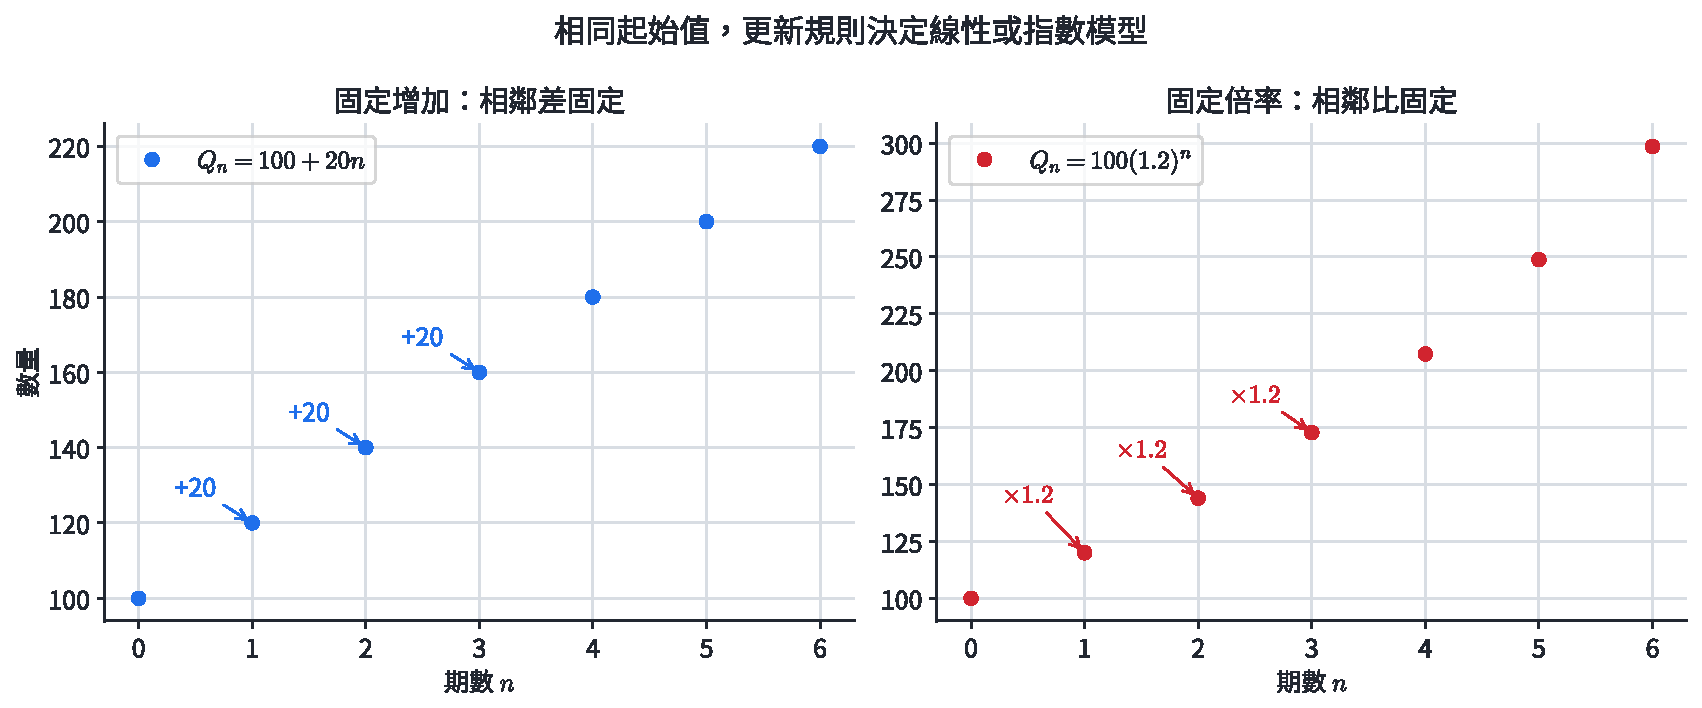
\includegraphics[width=0.94\linewidth,height=\textheight,keepaspectratio,alt={固定差與固定倍率形成的不同資料}]{assets/數B3-2-固定差與固定倍率.pdf}
\caption{固定差與固定倍率形成的不同資料}
\end{figure}

左圖相鄰點的高度差都是 \(20\)，對應線性模型 \(100+20n\)；右圖相鄰點的比值都是 \(1.2\)，對應指數模型 \(100(1.2)^n\)。資料中「差固定」與「比固定」是選擇模型的直接證據。

真實系統的倍率常會因資源不足、政策、溫度或個體差異而改變。指數模型適合倍率近似穩定的區間；超出該區間時，要用新資料重新估計參數。

\section{1. 指數函數的定義}\label{ux6307ux6578ux51fdux6578ux7684ux5b9aux7fa9}

\subsection{1.1 由固定倍率得到指數}\label{ux7531ux56faux5b9aux500dux7387ux5f97ux5230ux6307ux6578}

設初值為 \(Q_0\)，每一期乘上固定倍率 \(a\)，則

\[
Q_1=Q_0a,\qquad Q_2=Q_0a^2,\qquad Q_n=Q_0a^n.
\]

當期數擴張為實數變數 \(x\) 時，得到指數函數。\textbf{指數函數}定義為

\[
f(x)=a^x,\qquad a>0,\quad a\ne1.
\]

\begin{itemize}
\tightlist
\item
  \(a>0\) 使任意實數指數都能穩定定義；例如 \(a^{1/2}=\sqrt a\) 需要正的底數。
\item
  \(a\ne1\) 使函數會隨 \(x\) 變化；\(1^x\) 是恒等於 \(1\) 的常數函數。
\item
  定義域是所有實數，值域是所有正實數。
\end{itemize}

指數律

\[
a^{u+v}=a^ua^v,\qquad a^{u-v}=\frac{a^u}{a^v},\qquad (a^u)^v=a^{uv}
\]

是固定倍率能夠跨過多個時間間隔的代數基礎。

\subsection{例 1｜將百分率轉成更新倍率}\label{ux4f8b-1ux5c07ux767eux5206ux7387ux8f49ux6210ux66f4ux65b0ux500dux7387}

一個培養璿初有 \(400\) 個菌落，每小時增加 \(15\%\)。每小時更新倍率是 \(1+0.15=1.15\)，因此

\[
N_n=400(1.15)^n.
\]

\(3\) 小時後

\[
N_3=400(1.15)^3=608.35,
\]

若以完整個數記錄，約為 \(608\) 個菌落。

\subsection{例 2｜由隔期資料反求倍率與初值}\label{ux4f8b-2ux7531ux9694ux671fux8cc7ux6599ux53cdux6c42ux500dux7387ux8207ux521dux503c}

一組資料符合 \(Q_n=Q_0a^n\)，且 \(Q_2=360\)、\(Q_5=1215\)。兩式相除：

\[
\frac{Q_5}{Q_2}=a^3=\frac{1215}{360}=3.375=1.5^3.
\]

由 \(a>0\) 得 \(a=1.5\)，再代回：

\[
Q_0=\frac{360}{1.5^2}=160.
\]

所以 \(Q_n=160(1.5)^n\)。

\subsection{1.2 分節練習}\label{ux5206ux7bc0ux7df4ux7fd2}

\begin{enumerate}
\def\labelenumi{\arabic{enumi}.}
\tightlist
\item
  在 \(a=-2,\dfrac13,1,\sqrt5\) 中，選出可作為指數函數 \(f(x)=a^x\) 底數的數。
\item
  設 \(f(x)=4^x\)，求 \(f(-2)\)、\(f(1/2)\) 與 \(f(0)\)。
\item
  某量的資料依序為 \(250,300,360,432\)。若每期倍率固定，寫出以第一個數據為 \(Q_0\) 的模型。
\item
  一份材料的性能初值為 \(920\) 單位，每年保留前一年的 \(82\%\)。寫出 \(t\) 年後的模型，並求 \(3\) 年後的預測值。
\end{enumerate}

\subsection{1.3 分節練習解析}\label{ux5206ux7bc0ux7df4ux7fd2ux89e3ux6790}

\begin{enumerate}
\def\labelenumi{\arabic{enumi}.}
\tightlist
\item
  底數需滿足 \(a>0\) 且 \(a\ne1\)，所以可選 \(\dfrac13\) 與 \(\sqrt5\)。
\item
  \(f(-2)=1/16\)、\(f(1/2)=2\)、\(f(0)=1\)。
\item
  相鄰比值均為 \(1.2\)，因此 \(Q_n=250(1.2)^n\)。
\item
  \[
   Q(t)=920(0.82)^t,\qquad Q(3)=920(0.82)^3\approx507.2.
   \]
  預測值約為 \(507\) 單位，且低於初值，與保留率小於 \(1\) 一致。
\end{enumerate}

固定百分率變化會固定每期倍率，因此常用於短期人口、價格指數、折舊與設備效率模型。

\section{2. 指數函數的圖形與特徵}\label{ux6307ux6578ux51fdux6578ux7684ux5716ux5f62ux8207ux7279ux5fb5}

\subsection{2.1 底數決定增減}\label{ux5e95ux6578ux6c7aux5b9aux589eux6e1b}

對 \(f(x)=a^x\)、\(a>0\)且 \(a\ne1\)：

\begin{itemize}
\tightlist
\item
  圖形經過 \((0,1)\)，因為 \(a^0=1\)。
\item
  值域為 \((0,\infty)\)，直線 \(y=0\) 是水平漸近線。
\item
  \(a>1\) 時，\(x\) 每增加 \(1\)，函數值乘上 \(a>1\)，所以函數遞增。
\item
  \(0<a<1\) 時，\(x\) 每增加 \(1\)，函數值乘上小於 \(1\) 的正數，所以函數遞減。
\end{itemize}

\begin{figure}
\centering
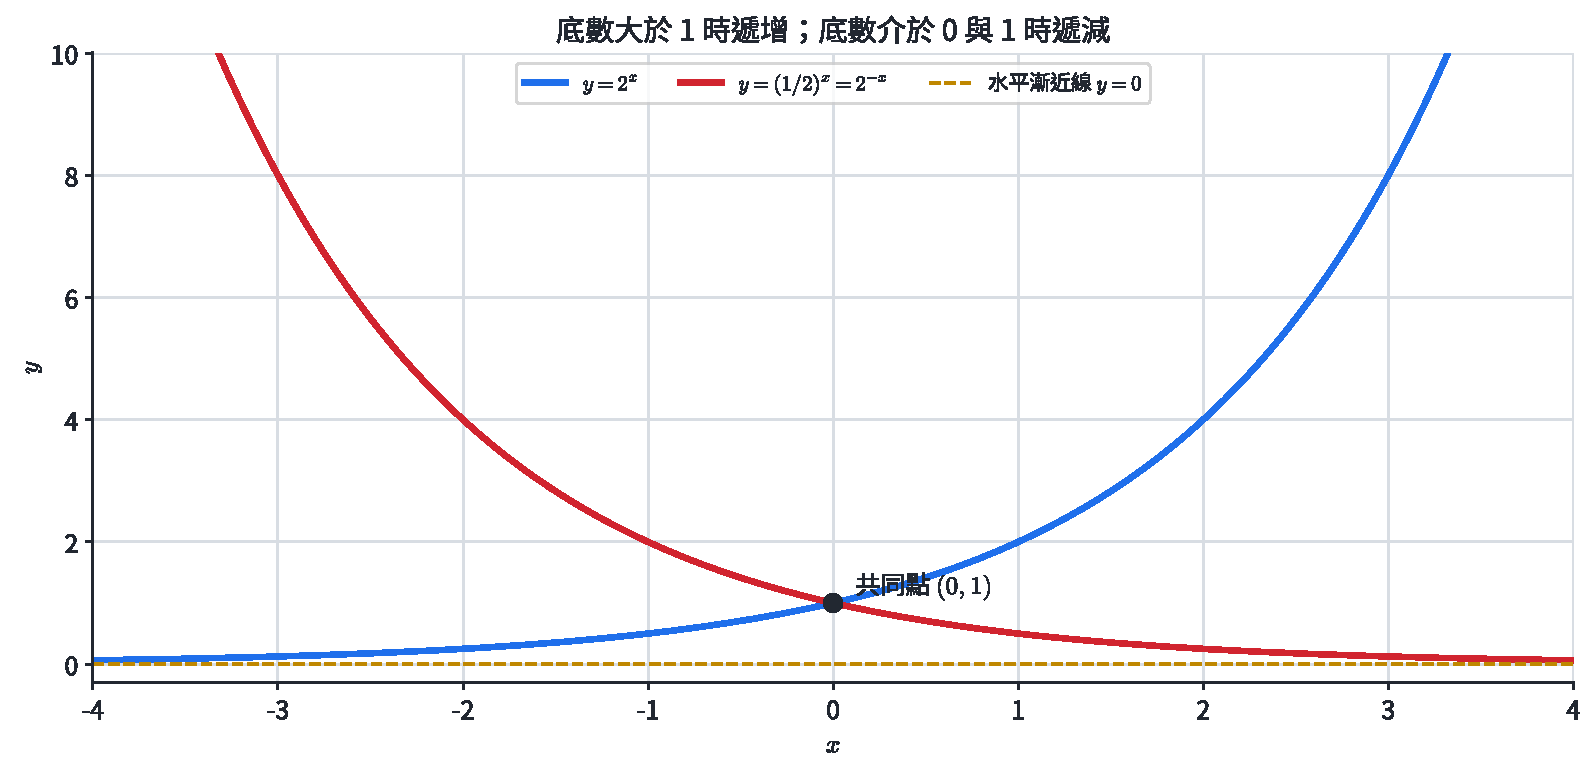
\includegraphics[width=0.9\linewidth,height=\textheight,keepaspectratio,alt={底數 2 與其倒數的指數圖形}]{assets/數B3-2-指數成長與衰退.pdf}
\caption{底數 2 與其倒數的指數圖形}
\end{figure}

圖中 \(y=2^x\) 與 \(y=(1/2)^x=2^{-x}\) 在 \(x=0\) 時都通過 \((0,1)\)，且兩圖關於 \(y\) 軸對稱。虛線 \(y=0\) 表示函數值可以任意接近 \(0\)，但仍保持為正。

\begin{figure}
\centering
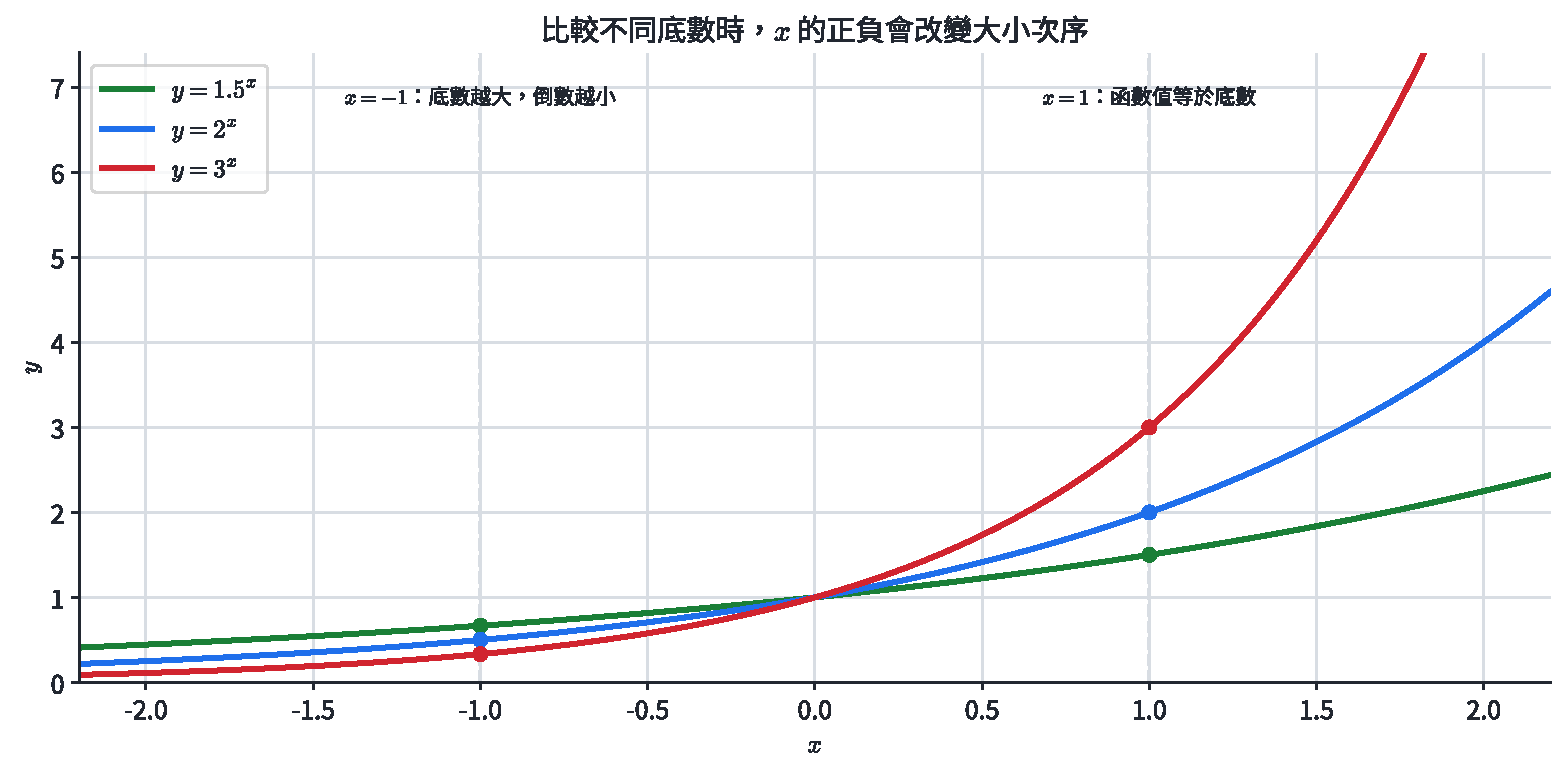
\includegraphics[width=0.9\linewidth,height=\textheight,keepaspectratio,alt={不同底數在正負指數時的大小次序}]{assets/數B3-2-指數底數比較.pdf}
\caption{不同底數在正負指數時的大小次序}
\end{figure}

在 \(x=1\) 時，底數越大函數值越大；在 \(x=-1\) 時，\(a^{-1}=1/a\)，大小次序因取倒數而反轉。

\subsection{2.2 指數方程式與不等式}\label{ux6307ux6578ux65b9ux7a0bux5f0fux8207ux4e0dux7b49ux5f0f}

當兩邊能改寫成相同底數時，利用單調性：

\[
a^u=a^v\Longleftrightarrow u=v.
\]

\[
\begin{aligned}
a>1 &: \quad a^u>a^v\Longleftrightarrow u>v,\\
0<a<1 &: \quad a^u>a^v\Longleftrightarrow u<v.
\end{aligned}
\]

若式子同時含有 \(a^{2x}\) 與 \(a^x\)，令 \(t=a^x>0\)，就能化為關於 \(t\) 的二次式。

\subsection{例 3｜比較指數數的大小}\label{ux4f8b-3ux6bd4ux8f03ux6307ux6578ux6578ux7684ux5927ux5c0f}

底數 \(1.7>1\)，函數 \(1.7^x\) 遞增。由 \(-0.4<1.2\)，可得

\[
1.7^{-0.4}<1.7^{1.2}.
\]

若底數改為 \(0.4\)，函數遞減，同一組指數得 \(0.4^{-0.4}>0.4^{1.2}\)。

\subsection{例 4｜將指數方程式化為同底}\label{ux4f8b-4ux5c07ux6307ux6578ux65b9ux7a0bux5f0fux5316ux70baux540cux5e95}

解 \(3^{2x-1}=27\)。由 \(27=3^3\)，且 \(3^x\) 一對一，得

\[
2x-1=3,\qquad x=2.
\]

代回左邊得 \(3^3=27\)，符合原式。

\subsection{例 5｜以換元求指數方程式}\label{ux4f8b-5ux4ee5ux63dbux5143ux6c42ux6307ux6578ux65b9ux7a0bux5f0f}

解 \(4^x-5\cdot2^x+4=0\)。令 \(t=2^x>0\)，則 \(4^x=t^2\)：

\[
t^2-5t+4=(t-1)(t-4)=0.
\]

\(t=1,4\) 皆為正，分別得 \(x=0,2\)。

\begin{figure}
\centering
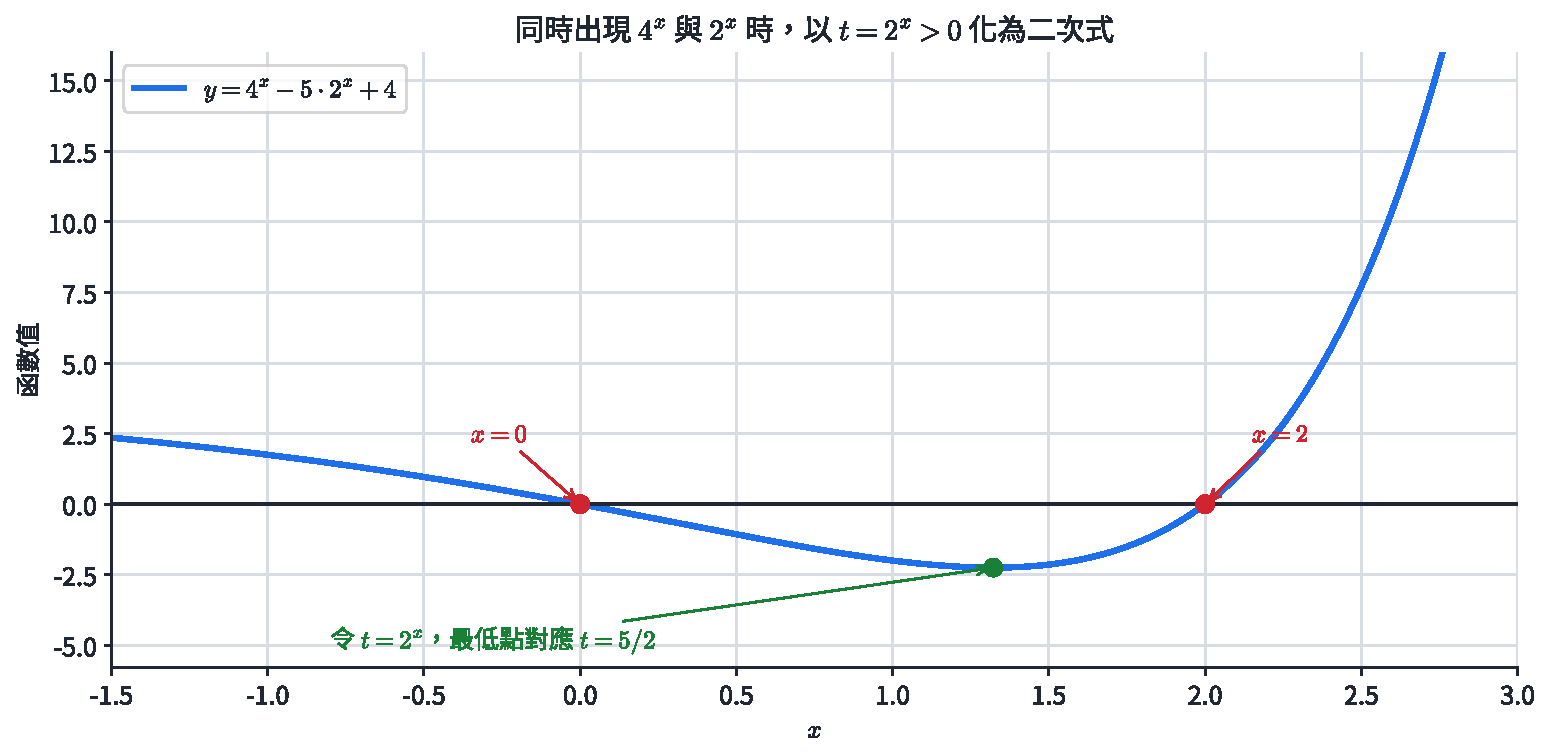
\includegraphics[width=0.88\linewidth,height=\textheight,keepaspectratio,alt={換元後的二次式與原指數函數交點}]{assets/數B3-2-指數換元與交點.pdf}
\caption{換元後的二次式與原指數函數交點}
\end{figure}

圖上兩個 \(x\) 軸交點正是 \(x=0,2\)；圖中最低點對應 \(t=2^x=5/2\)，也與二次式的對稱軸一致。

\subsection{例 6｜底數小於 1 的指數不等式}\label{ux4f8b-6ux5e95ux6578ux5c0fux65bc-1-ux7684ux6307ux6578ux4e0dux7b49ux5f0f}

解 \(\left(\dfrac12\right)^{x-1}\ge8\)。將 \(8\) 改寫為 \(\left(\dfrac12\right)^{-3}\)。因底數介於 \(0\) 與 \(1\)，函數遞減：

\[
x-1\le-3,\qquad x\le-2.
\]

\subsection{2.3 分節練習}\label{ux5206ux7bc0ux7df4ux7fd2-1}

\begin{enumerate}
\def\labelenumi{\arabic{enumi}.}
\tightlist
\item
  寫出 \(y=5^x\) 的定義域、值域、通過的固定點與增減性。
\item
  比較 \(2.3^{-1.4}\) 與 \(2.3^{-0.6}\)，再比較 \(0.3^{-1.4}\) 與 \(0.3^{-0.6}\)。
\item
  解 \(5^{3x+1}=125^{x-1}\)。
\item
  解 \(9^x-10\cdot3^x+9=0\)。
\item
  解 \(4^{2x-1}<8^{x+1}\)。
\end{enumerate}

\subsection{2.4 分節練習解析}\label{ux5206ux7bc0ux7df4ux7fd2ux89e3ux6790-1}

\begin{enumerate}
\def\labelenumi{\arabic{enumi}.}
\tightlist
\item
  定義域為 \(\mathbb R\)，值域為 \((0,\infty)\)，通過 \((0,1)\)，且在整個定義域遞增。
\item
  \(2.3^x\) 遞增，所以 \(2.3^{-1.4}<2.3^{-0.6}\)；\(0.3^x\) 遞減，所以 \(0.3^{-1.4}>0.3^{-0.6}\)。
\item
  \(125=5^3\)，得 \(3x+1=3x-3\)，這導致 \(1=-3\)，故無實數解。
\item
  令 \(t=3^x>0\)，得 \((t-1)(t-9)=0\)，因此 \(x=0,2\)。
\item
  改寫成 \(2^{4x-2}<2^{3x+3}\)。因 \(2^x\) 遞增，得 \(4x-2<3x+3\)，所以 \(x<5\)。
\end{enumerate}

指數圖形把「倍率」轉成「高度」。圖形增減、與水平線的交點和是否超過門檻，都能直接對應方程式或不等式。

\section{3. 指數的應用：成長、衰退、單利與複利}\label{ux6307ux6578ux7684ux61c9ux7528ux6210ux9577ux8870ux9000ux55aeux5229ux8207ux8907ux5229}

\subsection{3.1 固定時間間隔的模型}\label{ux56faux5b9aux6642ux9593ux9593ux9694ux7684ux6a21ux578b}

設初值為 \(Q_0\)，每 \(h\) 單位時間乘上 \(b\)，經過 \(t\) 單位時間時，相當於經過 \(t/h\) 個間隔：

\[
Q(t)=Q_0b^{t/h}.
\]

\begin{itemize}
\tightlist
\item
  每期成長率為 \(r\) 時，\(b=1+r>1\)。
\item
  每期衰退率為 \(r\) 時，\(b=1-r\)，且 \(0<b<1\)。
\item
  半衰期為 \(h\) 時，\(b=1/2\)，所以 \(Q(t)=Q_0(1/2)^{t/h}\)。
\end{itemize}

\begin{figure}
\centering
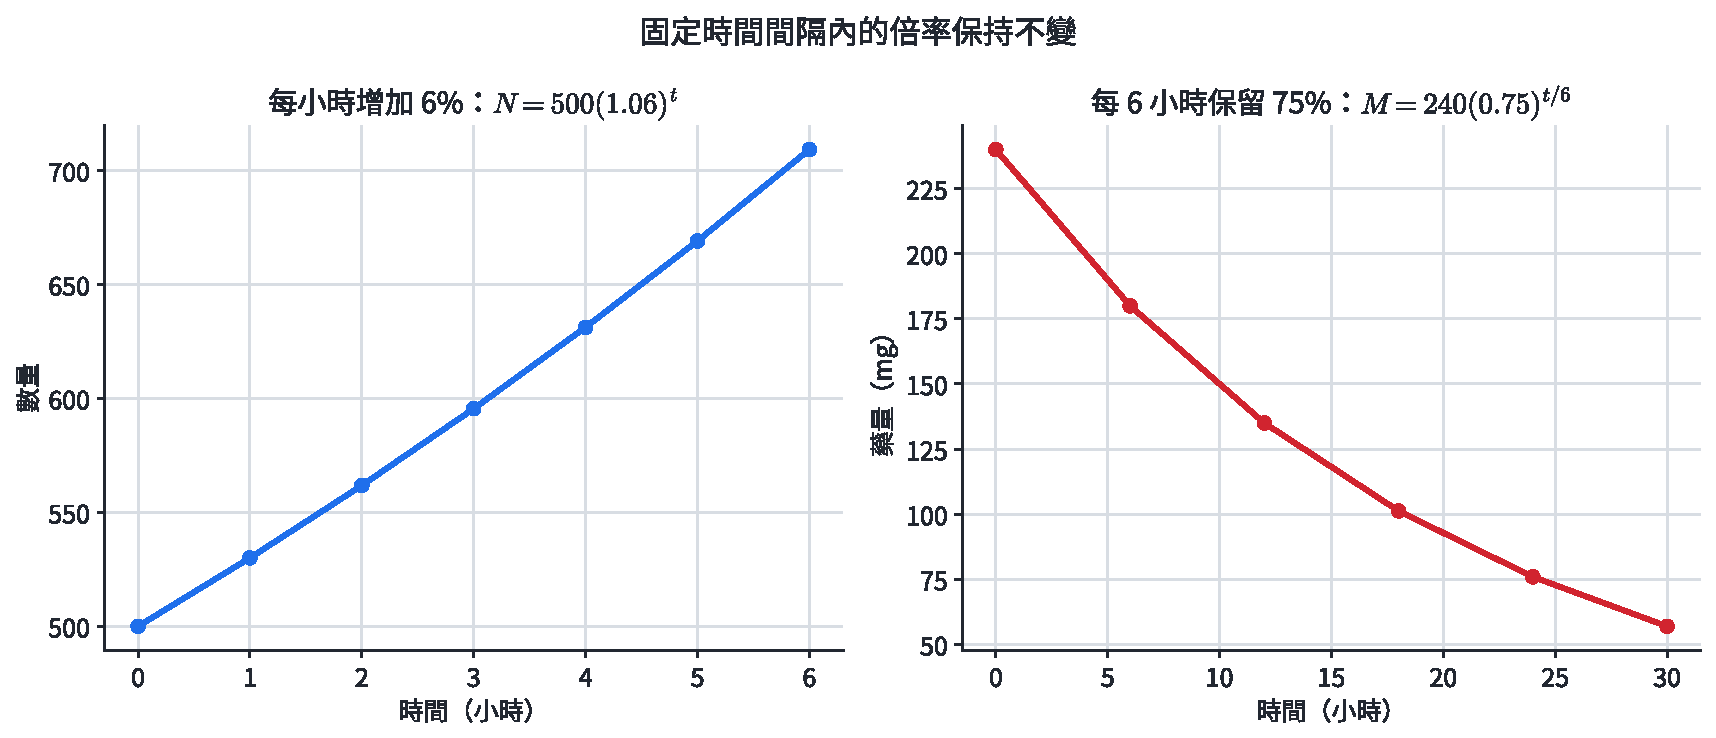
\includegraphics[width=0.94\linewidth,height=\textheight,keepaspectratio,alt={成長與衰退資料的固定時間倍率}]{assets/數B3-2-成長衰退資料.pdf}
\caption{成長與衰退資料的固定時間倍率}
\end{figure}

左圖每相隔 \(1\) 小時的比值為 \(1.06\)；右圖每相隔 \(6\) 小時的比值為 \(0.75\)。時間單位與倍率的間隔需配對，所以右圖指數是 \(t/6\)。

\subsection{3.2 單利與複利}\label{ux55aeux5229ux8207ux8907ux5229}

本金為 \(P\)，每期利率為 \(r\)，經過 \(n\) 期：

\begin{itemize}
\tightlist
\item
  \textbf{單利}每期只以原本金計息，每期增加固定金額 \(Pr\)：\(A=P(1+nr)\)。
\item
  \textbf{複利}每期將當期本利和作為下期本金，每期乘上 \(1+r\)：\(A=P(1+r)^n\)。
\end{itemize}

\begin{figure}
\centering
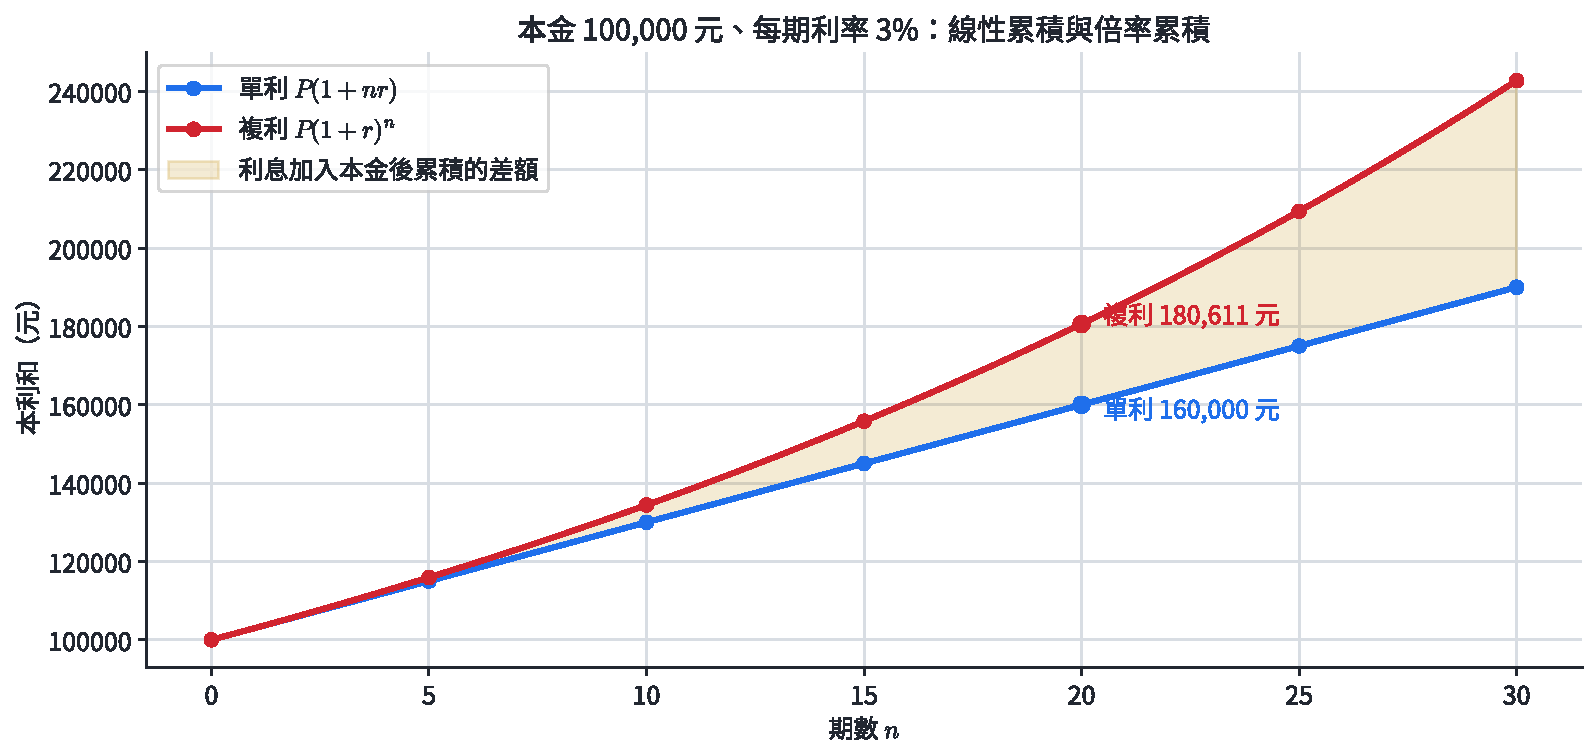
\includegraphics[width=0.9\linewidth,height=\textheight,keepaspectratio,alt={同一本金與利率下的單利、複利累積}]{assets/數B3-2-單利與複利.pdf}
\caption{同一本金與利率下的單利、複利累積}
\end{figure}

圖中兩模型起於同一本金。單利每年增加同一金額，圖形是直線；複利的利息也進入下一期本金，所以差距會隨時間擴大。

\subsection{例 7｜每小時成長的菌落}\label{ux4f8b-7ux6bcfux5c0fux6642ux6210ux9577ux7684ux83ccux843d}

菌落初始數為 \(500\)，每小時增加 \(6\%\)。在環境與資源近似不變的前 \(8\) 小時，模型為

\[
N(t)=500(1.06)^t,\qquad0\le t\le8.
\]

\[
N(6)=500(1.06)^6\approx709.3.
\]

所以 \(6\) 小時後預測約 \(709\) 個菌落。式中的時間區間記錄模型所依據的環境條件。

\subsection{例 8｜不同時間單位的藥物保留率}\label{ux4f8b-8ux4e0dux540cux6642ux9593ux55aeux4f4dux7684ux85e5ux7269ux4fddux7559ux7387}

人體中某藥物初始量為 \(240\text{ mg}\)，每 \(6\) 小時保留 \(75\%\)。\(24\) 小時包含 \(4\) 個間隔，因此

\[
M(24)=240(0.75)^4=75.9375\text{ mg}.
\]

預測約為 \(75.9\text{ mg}\)，為正且小於初始量，與保留率一致。

\subsection{例 9｜單利與複利的數值差異}\label{ux4f8b-9ux55aeux5229ux8207ux8907ux5229ux7684ux6578ux503cux5deeux7570}

本金 \(100{,}000\) 元，年利率 \(3\%\)，比較 \(10\) 年單利與每年複利的本利和。

\[
A_s=100000(1+10\times0.03)=130000,
\]

\[
A_c=100000(1.03)^{10}\approx134391.64.
\]

複利多出約 \(4391.64\) 元，這部分來自過去利息在後續期間繼續生息。

\subsection{例 10｜一年複利多次的模型}\label{ux4f8b-10ux4e00ux5e74ux8907ux5229ux591aux6b21ux7684ux6a21ux578b}

投資 \(80{,}000\) 元，名義年利率 \(4\%\)，每半年複利一次。每期利率為 \(0.04/2=0.02\)，\(5\) 年共 \(10\) 期，所以

\[
A=80000(1.02)^{10}\approx97519.55.
\]

本利和約為 \(97{,}520\) 元。

\subsection{3.3 分節練習}\label{ux5206ux7bc0ux7df4ux7fd2-2}

\begin{enumerate}
\def\labelenumi{\arabic{enumi}.}
\tightlist
\item
  某城市人口為 \(80{,}000\)，短期內每年增加 \(1.8\%\)。寫出模型並估計 \(5\) 年後人口。
\item
  某同位素半衰期為 \(12\) 年，初始質量 \(64\text{ g}\)。求 \(30\) 年後質量。
\item
  一種藥物初始量為 \(300\text{ mg}\)，\(4\) 小時後為 \(210\text{ mg}\)。若每 \(4\) 小時保留率固定，求 \(12\) 小時後的量。
\item
  本金 \(50{,}000\) 元以年利率 \(2.4\%\) 計息，求 \(8\) 年單利本利和。
\item
  本金 \(120{,}000\) 元，名義年利率 \(3.6\%\)，每季複利。求 \(6\) 年後本利和。
\item
  一種植物在溫室前 \(10\) 天呈固定倍率成長，第 \(0,2,4\) 天高度為 \(5,7.2,10.368\text{ cm}\)。建立模型，並說明將它用來預測第 \(100\) 天時需要哪一類額外證據。
\end{enumerate}

\subsection{3.4 分節練習解析}\label{ux5206ux7bc0ux7df4ux7fd2ux89e3ux6790-2}

\begin{enumerate}
\def\labelenumi{\arabic{enumi}.}
\tightlist
\item
  \(P(t)=80000(1.018)^t\)，且 \(P(5)\approx87464\)，約 \(87{,}464\) 人。
\item
  \(M(t)=64(1/2)^{t/12}\)，所以 \(M(30)=64(1/2)^{2.5}\approx11.31\text{ g}\)。
\item
  每 \(4\) 小時保留率為 \(0.7\)，所以 \(M(12)=300(0.7)^3=102.9\text{ mg}\)。
\item
  \(A=50000(1+8\times0.024)=59600\) 元。
\item
  每季利率為 \(0.009\)，總期數為 \(24\)，所以 \(A=120000(1.009)^{24}\approx148788.46\) 元。
\item
  每 \(2\) 天倍率均為 \(1.44\)，故 \(H(t)=5(1.44)^{t/2}\)，\(0\le t\le10\)。要外推到第 \(100\) 天，需要長期資料證明光照、水分、空間與植物成熟後的成長倍率仍近似不變。
\end{enumerate}

\section{4. 常用對數的定義與性質}\label{ux5e38ux7528ux5c0dux6578ux7684ux5b9aux7fa9ux8207ux6027ux8cea}

\subsection{4.1 對數是所需的指數}\label{ux5c0dux6578ux662fux6240ux9700ux7684ux6307ux6578}

\textbf{常用對數}以 \(10\) 為底，寫作 \(\log x\)：

\[
10^y=x\Longleftrightarrow y=\log x,\qquad x>0.
\]

例如 \(10^3=1000\)，所以 \(\log1000=3\)；\(10^{-2}=0.01\)，所以 \(\log0.01=-2\)。真數 \(x\) 必須為正，這來自 \(10^y\) 的值域 \((0,\infty)\)。

\begin{figure}
\centering
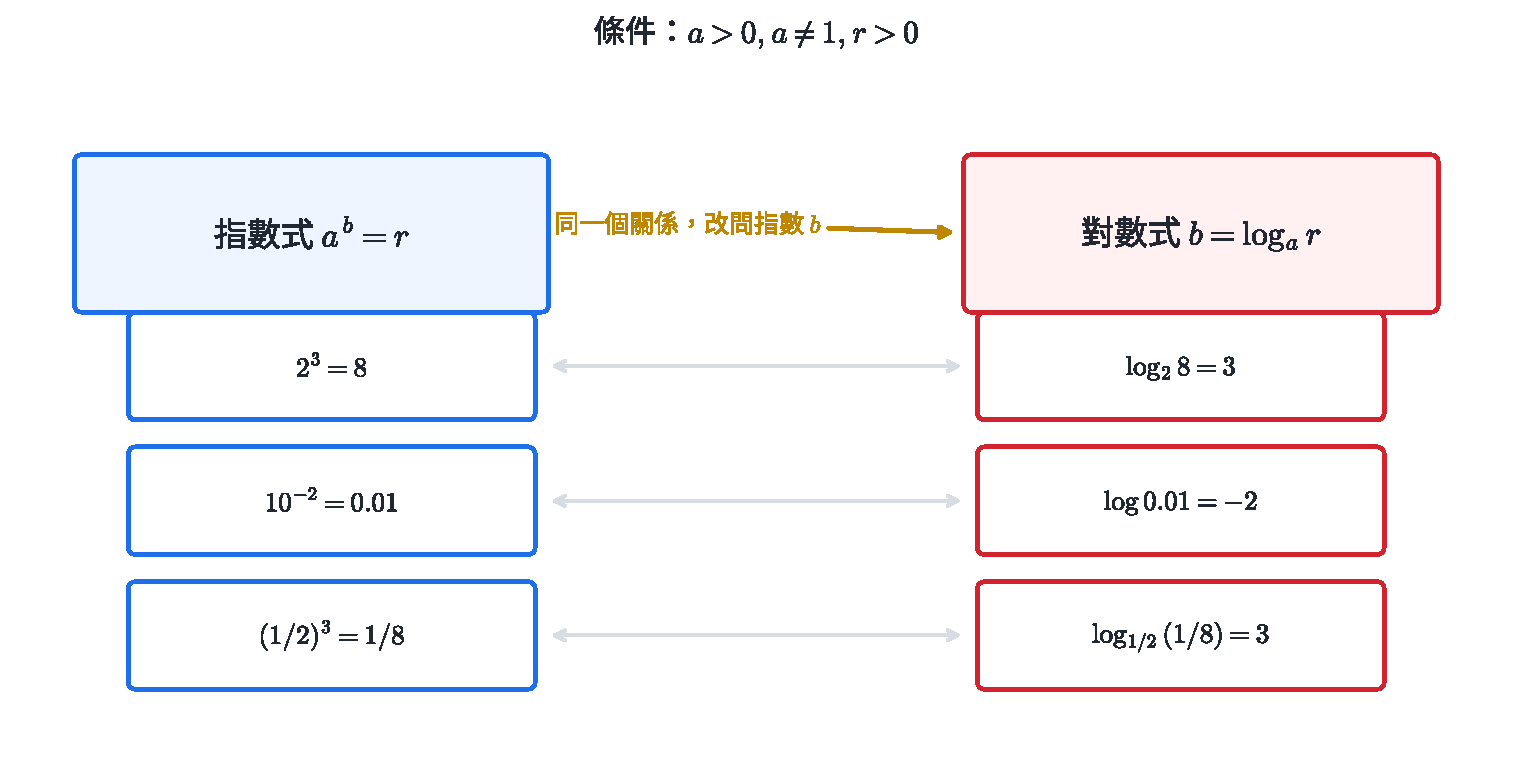
\includegraphics[width=0.88\linewidth,height=\textheight,keepaspectratio,alt={同一關係的指數形式與對數形式}]{assets/數B3-2-指數與對數對照.pdf}
\caption{同一關係的指數形式與對數形式}
\end{figure}

圖中每一列都在說同一件事：左側提供底數、指數與結果，右側把結果放進對數，取回原來的指數。

\subsection{4.2 對數律與推導}\label{ux5c0dux6578ux5f8bux8207ux63a8ux5c0e}

對正數 \(M,N\) 與實數 \(r\)：

\[
\log(MN)=\log M+\log N,\qquad
\log\frac{M}{N}=\log M-\log N,\qquad
\log(M^r)=r\log M.
\]

令 \(u=\log M\)、\(v=\log N\)，則 \(M=10^u\)、\(N=10^v\)，所以

\[
MN=10^u10^v=10^{u+v}.
\]

由定義得 \(\log(MN)=u+v=\log M+\log N\)。商法律與冪法律同樣來自指數律。

\begin{figure}
\centering
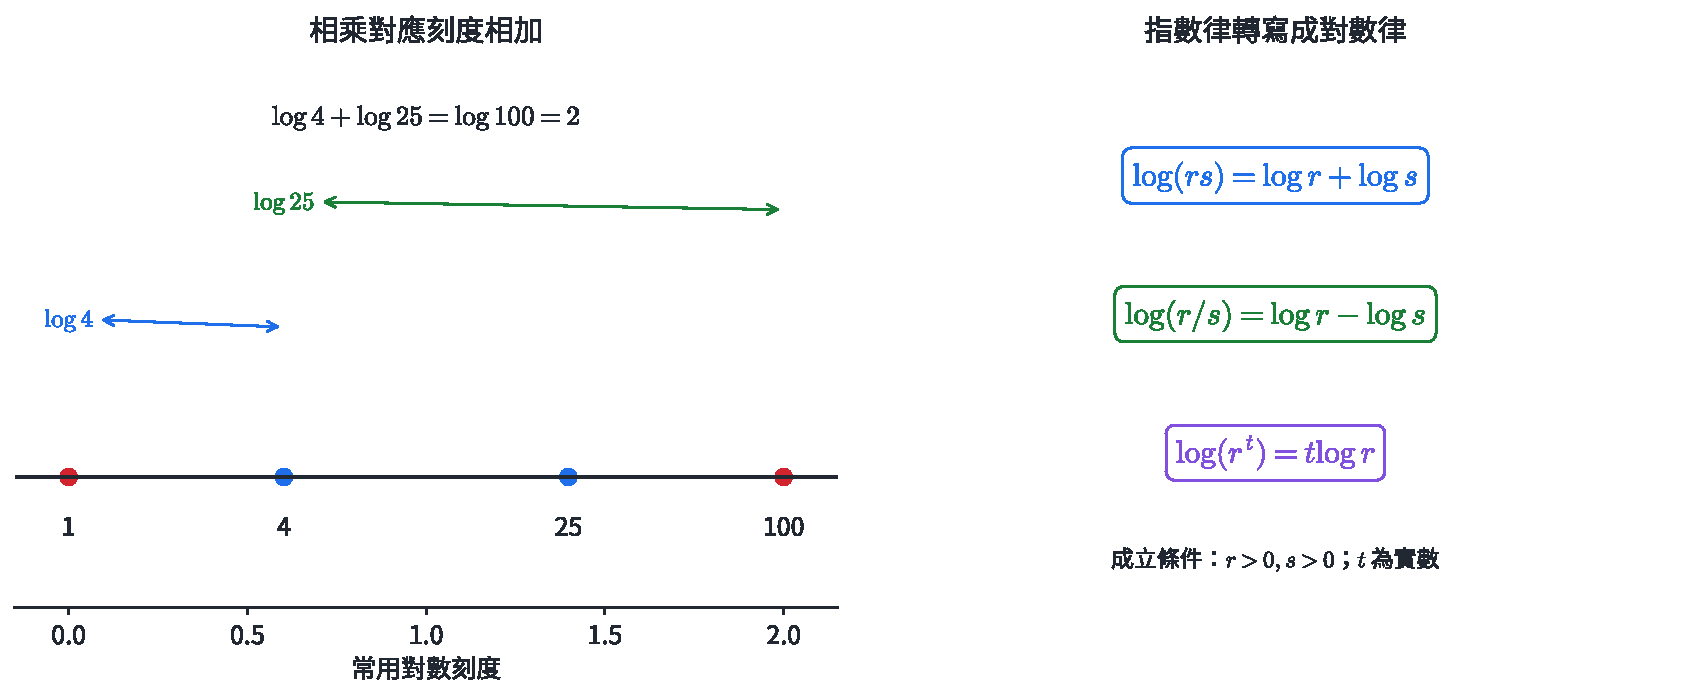
\includegraphics[width=0.9\linewidth,height=\textheight,keepaspectratio,alt={對數將乘法倍率轉成加法距離}]{assets/數B3-2-對數律刻度.pdf}
\caption{對數將乘法倍率轉成加法距離}
\end{figure}

圖中數量從 \(1\) 乘上 \(10\) 到 \(10\)，再乘上 \(10\) 到 \(100\)；取常用對數後，座標從 \(0\) 加 \(1\) 到 \(1\)，再加 \(1\) 到 \(2\)。

\subsection{例 11｜從指數值讀出常用對數}\label{ux4f8b-11ux5f9eux6307ux6578ux503cux8b80ux51faux5e38ux7528ux5c0dux6578}

由 \(100000=10^5\)、\(0.001=10^{-3}\)、\(\sqrt{10}=10^{1/2}\)，得

\[
\log100000=5,\qquad \log0.001=-3,\qquad \log\sqrt{10}=\frac12.
\]

\subsection{例 12｜用對數律合併運算}\label{ux4f8b-12ux7528ux5c0dux6578ux5f8bux5408ux4f75ux904bux7b97}

已知 \(\log2\approx0.3010\)、\(\log3\approx0.4771\)，求 \(\log72\)。因 \(72=2^3\cdot3^2\)，所以

\[
\log72=3\log2+2\log3\approx1.8572.
\]

\(10<72<100\)，所以 \(1<\log72<2\)，結果位於合理區間。

\subsection{例 13｜用科學記號讀取數量級}\label{ux4f8b-13ux7528ux79d1ux5b78ux8a18ux865fux8b80ux53d6ux6578ux91cfux7d1a}

設 \(x=4.7\times10^6\)，則

\[
\log x=\log4.7+6.
\]

因 \(1<4.7<10\)，有 \(0<\log4.7<1\)，所以 \(6<\log x<7\)。這表示 \(x\) 位於 \(10^6\) 與 \(10^7\) 之間，也就是七位數。

\subsection{4.3 分節練習}\label{ux5206ux7bc0ux7df4ux7fd2-3}

\begin{enumerate}
\def\labelenumi{\arabic{enumi}.}
\tightlist
\item
  求 \(\log10^7\)、\(\log10^{-4}\) 與 \(\log\sqrt[3]{100}\)。
\item
  將 \(\log5+\log8-\log2\) 合併成一個對數並求值。
\item
  已知 \(\log2\approx0.3010\)，求 \(\log40\)、\(\log0.08\)。
\item
  化簡 \(2\log3+\dfrac12\log16-\log12\)。
\item
  設 \(x=7.2\times10^{-5}\)，寫出 \(\log x\) 與 \(\log7.2\) 的關係，並判斷 \(\log x\) 介於哪兩個相鄰整數之間。
\end{enumerate}

\subsection{4.4 分節練習解析}\label{ux5206ux7bc0ux7df4ux7fd2ux89e3ux6790-3}

\begin{enumerate}
\def\labelenumi{\arabic{enumi}.}
\tightlist
\item
  \(\log10^7=7\)、\(\log10^{-4}=-4\)、\(\log\sqrt[3]{100}=2/3\)。
\item
  \(\log5+\log8-\log2=\log20=1+\log2\approx1.3010\)。
\item
  \(\log40=2\log2+1\approx1.6020\)；\(\log0.08=3\log2-2\approx-1.0970\)。
\item
  \[
   2\log3+\frac12\log16-\log12
   =\log\frac{3^2\sqrt{16}}{12}=\log3.
   \]
\item
  \(\log x=\log7.2-5\)。因 \(0<\log7.2<1\)，所以 \(-5<\log x<-4\)。
\end{enumerate}

對數律把乘法、除法與冪次轉成加法、減法與倍數，這是對數可以壓縮尺度、線性化指數資料的原因。

\section{5. 一般對數、換底與計算}\label{ux4e00ux822cux5c0dux6578ux63dbux5e95ux8207ux8a08ux7b97}

\subsection{5.1 一般對數的定義}\label{ux4e00ux822cux5c0dux6578ux7684ux5b9aux7fa9}

設

\[
a>0,\qquad a\ne1,\qquad r>0.
\]

若 \(a^b=r\)，則定義

\[
b=\log_a r.
\]

底數 \(a\) 決定用哪一組指數刻度，真數 \(r\) 是指數函數的正值，對數值 \(b\) 是從底數到真數所需的指數。特別地，

\[
\log_a1=0,\qquad \log_aa=1.
\]

一般對數也滿足乘法、商與冪的對數律，條件同樣是各真數為正。

\subsection{5.2 換底公式}\label{ux63dbux5e95ux516cux5f0f}

令 \(x=\log_a r\)，則 \(a^x=r\)。對等式兩邊取以 \(c\) 為底的對數：

\[
x\log_c a=\log_c r.
\]

因此

\[
\boxed{\log_a r=\frac{\log_c r}{\log_c a}},
\]

其中 \(c>0\)、\(c\ne1\)。電子計算器通常提供 \(\log\) 與 \(\ln\)，換底公式讓任意底數的對數都能使用這兩個鍵計算。

\subsection{例 14｜在指數形式與對數形式間轉換}\label{ux4f8b-14ux5728ux6307ux6578ux5f62ux5f0fux8207ux5c0dux6578ux5f62ux5f0fux9593ux8f49ux63db}

由 \(3^4=81\)，得

\[
\log_3 81=4.
\]

由 \(2^{-3}=1/8\)，得

\[
\log_2\frac18=-3.
\]

反向地，\(\log_5 125=3\) 與 \(5^3=125\) 是同一個數量關係的兩種寫法。

\subsection{例 15｜用換底公式計算任意底數}\label{ux4f8b-15ux7528ux63dbux5e95ux516cux5f0fux8a08ux7b97ux4efbux610fux5e95ux6578}

求 \(\log_8 20\)。取常用對數換底：

\[
\log_8 20=\frac{\log20}{\log8}\approx1.4406.
\]

因 \(8^1<20<8^2\)，故答案介於 \(1\) 與 \(2\) 之間，與計算值一致。

\subsection{例 16｜對數求解無法化成同底的指數方程式}\label{ux4f8b-16ux5c0dux6578ux6c42ux89e3ux7121ux6cd5ux5316ux6210ux540cux5e95ux7684ux6307ux6578ux65b9ux7a0bux5f0f}

解 \(5^x=17\)。兩邊取常用對數：

\[
\log(5^x)=\log17,\qquad x\log5=\log17.
\]

因此

\[
x=\frac{\log17}{\log5}=\log_5 17\approx1.7604.
\]

\(5^1<17<5^2\)，所以 \(1<x<2\)，對應原函數的遞增性。

\subsection{5.3 分節練習}\label{ux5206ux7bc0ux7df4ux7fd2-4}

\begin{enumerate}
\def\labelenumi{\arabic{enumi}.}
\tightlist
\item
  求 \(\log_2 32\)、\(\log_3(1/27)\)、\(\log_{1/2}8\)。
\item
  將 \(7^{-2}=1/49\) 寫成對數形式，並將 \(\log_4 64=3\) 寫成指數形式。
\item
  用換底公式求 \(\log_7 30\)，答案取到小數點後四位。
\item
  化簡 \((\log_2 3)(\log_3 5)(\log_5 16)\)。
\item
  解 \(7^{2x-1}=20\)，以對數表示精確解，再求近似值。
\end{enumerate}

\subsection{5.4 分節練習解析}\label{ux5206ux7bc0ux7df4ux7fd2ux89e3ux6790-4}

\begin{enumerate}
\def\labelenumi{\arabic{enumi}.}
\tightlist
\item
  \[
   \log_2 32=5,\qquad \log_3\frac1{27}=-3,\qquad
   \log_{1/2}8=-3.
   \]
\item
  \(7^{-2}=1/49\) 可寫為 \(\log_7(1/49)=-2\)；\(\log_4 64=3\) 可寫為 \(4^3=64\)。
\item
  \[
   \log_7 30=\frac{\log30}{\log7}\approx1.7479.
   \]
  \(7^1<30<7^2\)，所以近似值介於 \(1\) 與 \(2\)。
\item
  以換底公式約分：
  \[
  \frac{\log3}{\log2}\cdot\frac{\log5}{\log3}\cdot
  \frac{\log16}{\log5}
  =\frac{\log16}{\log2}=\log_2 16=4.
  \]
\item
  \[
   (2x-1)\log7=\log20,\qquad
   x=\frac12\left(1+\frac{\log20}{\log7}\right)\approx1.2698.
   \]
\end{enumerate}

換底公式把對數定義轉成可計算的比值。它用於反求成長時間、半衰期、未知利率與任意底數的尺度。

\section{6. 對數的應用：時間、自然底數與對數尺度}\label{ux5c0dux6578ux7684ux61c9ux7528ux6642ux9593ux81eaux7136ux5e95ux6578ux8207ux5c0dux6578ux5c3aux5ea6}

\subsection{6.1 反求時間與 72 法則}\label{ux53cdux6c42ux6642ux9593ux8207-72-ux6cd5ux5247}

對成長模型 \(Q(t)=Q_0a^t\)，若要找到達成目標 \(Q_*\) 的時間，由

\[
Q_0a^t=Q_*
\]

取對數得

\[
t=\frac{\log(Q_*/Q_0)}{\log a}.
\]

年成長率為 \(p\%\) 時，翻倍時間的精確模型是

\[
T=\frac{\log2}{\log(1+p/100)}.
\]

當 \(p\) 位於常見的單位數百分率區間時，\(T\approx72/p\) 是便於心算的近似，精確值仍由上式決定。

\subsection{例 17｜翻倍時間與 72 法則}\label{ux4f8b-17ux7ffbux500dux6642ux9593ux8207-72-ux6cd5ux5247}

年複合成長率為 \(6\%\)。精確翻倍時間為

\[
T=\frac{\log2}{\log1.06}\approx11.90\text{ 年}.
\]

\(72/6=12\) 年，與精確模型相差約 \(0.10\) 年，適合用來快速估計。

\subsection{\texorpdfstring{6.2 複利頻率與自然底數 \(e\)}{6.2 複利頻率與自然底數 e}}\label{ux8907ux5229ux983bux7387ux8207ux81eaux7136ux5e95ux6578-e}

本金 \(1\) 元、年利率 \(100\%\)，一年複利 \(n\) 次時，年底金額為

\[
\left(1+\frac1n\right)^n.
\]

當複利次數 \(n\) 不斷增加，這串數越來越接近一個常數：

\[
e=\lim_{n\to\infty}\left(1+\frac1n\right)^n\approx2.71828.
\]

\begin{figure}
\centering
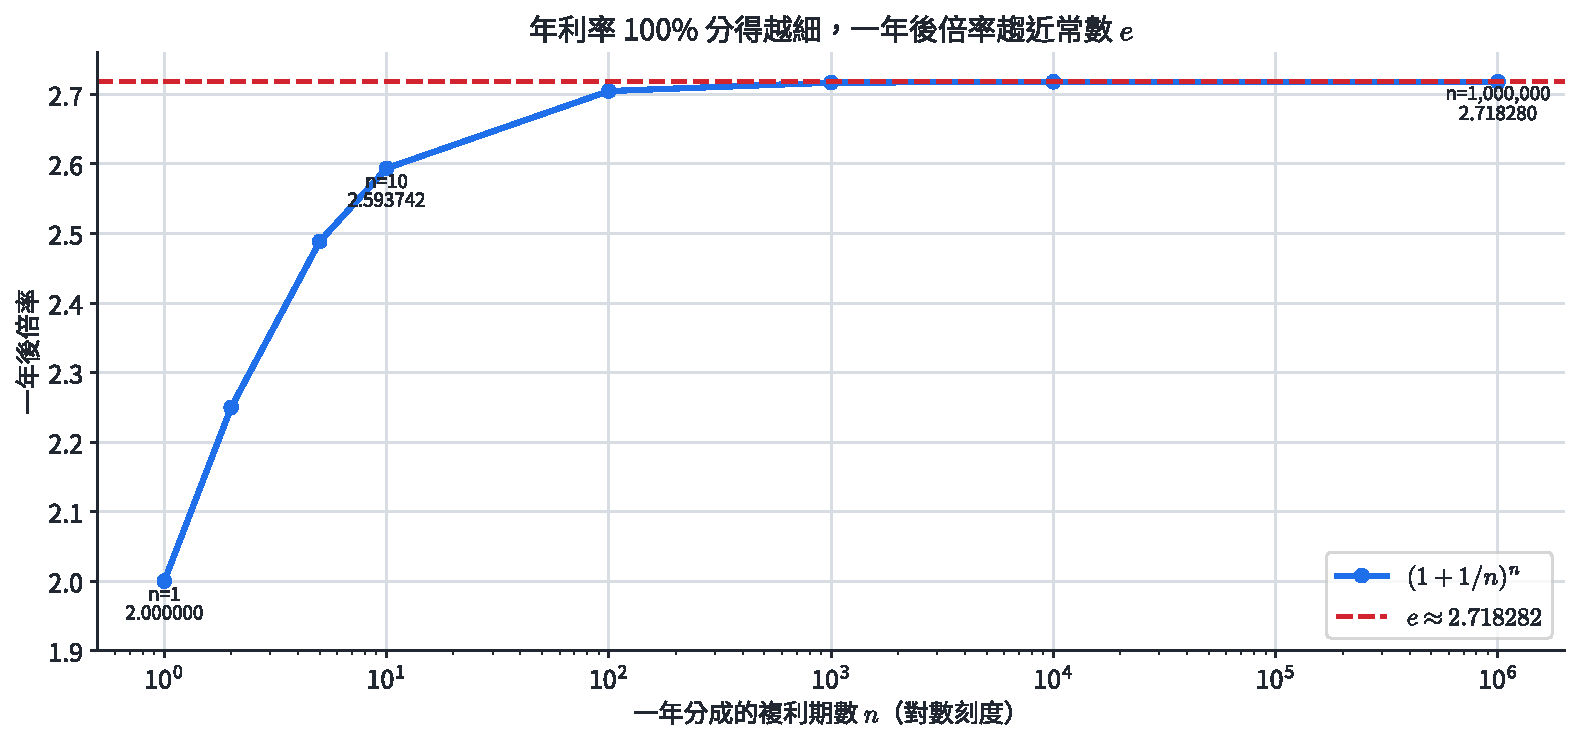
\includegraphics[width=0.9\linewidth,height=\textheight,keepaspectratio,alt={複利頻率增加時數值趨近常數 e}]{assets/數B3-2-複利頻率與常數e.pdf}
\caption{複利頻率增加時數值趨近常數 e}
\end{figure}

圖中點列隨 \(n\) 增加而接近水平線 \(y=e\)。以 \(e\) 為底的對數稱為\textbf{自然對數}，記作

\[
\ln x=\log_e x,\qquad x>0.
\]

連續成長率為 \(r\) 、時間為 \(t\) 時，模型常寫成 \(Q(t)=Q_0e^{rt}\)。

\subsection{例 18｜連續複利}\label{ux4f8b-18ux9023ux7e8cux8907ux5229}

本金 \(50{,}000\) 元以年利率 \(2.5\%\) 連續複利 \(6\) 年，則

\[
A=50000e^{0.025\times6}
=50000e^{0.15}\approx58091.71.
\]

本利和約為 \(58{,}092\) 元。

\subsection{6.3 分貝、pH 與地震規模}\label{ux5206ux8c9dph-ux8207ux5730ux9707ux898fux6a21}

對數尺度適合數值橫跨多個數量級、且倍數差比絕對差更有意義的量。

\begin{itemize}
\tightlist
\item
  聲強級：\(D=10\log(I/I_0)\) 分貝，\(I>0\)。
\item
  酸鹼值：\(\mathrm{pH}=-\log[\mathrm H^+]\)，\([\mathrm H^+]>0\)，濃度以 \(\mathrm{mol/L}\) 計。
\item
  地震能量與規模的常用模型：\(\log E=11.8+1.5M\)，其中 \(E\) 以爾格計。
\end{itemize}

\begin{figure}
\centering
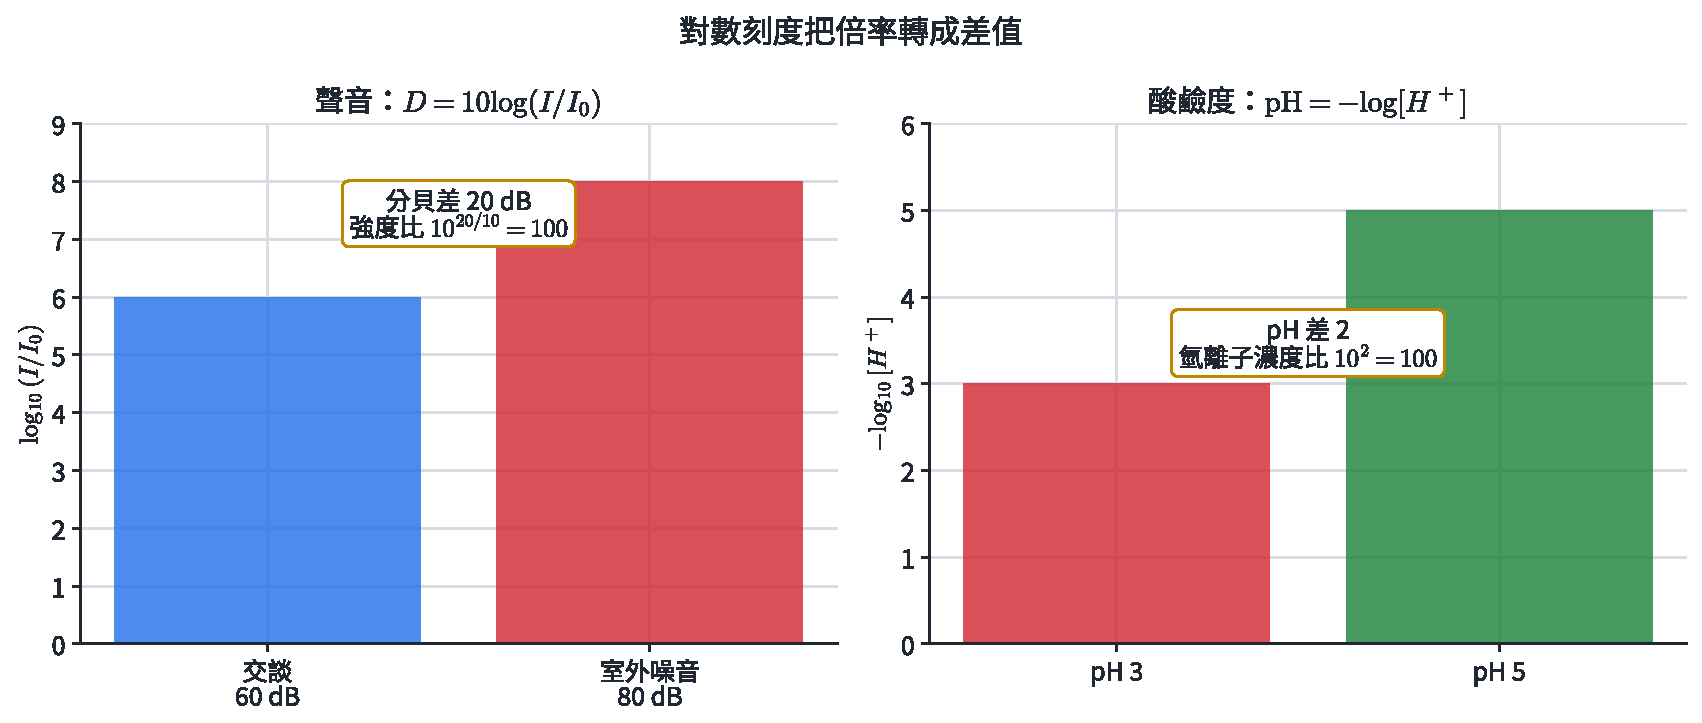
\includegraphics[width=0.94\linewidth,height=\textheight,keepaspectratio,alt={聲強與氫離子濃度在對數尺度上的對應}]{assets/數B3-2-對數尺度.pdf}
\caption{聲強與氫離子濃度在對數尺度上的對應}
\end{figure}

圖中聲強比每乘 \(10\)，分貝增加 \(10\)；氫離子濃度每乘 \(10\)，pH 減少 \(1\)。符號差異來自 pH 定義前的負號。

\subsection{例 19｜分貝差轉回聲強倍率}\label{ux4f8b-19ux5206ux8c9dux5deeux8f49ux56deux8072ux5f37ux500dux7387}

兩聲音的聲強分別為 \(I_1,I_2\)，聲強級相差 \(30\) 分貝。由

\[
30=10\log\frac{I_2}{I_1}
\]

得

\[
\log\frac{I_2}{I_1}=3,\qquad
\frac{I_2}{I_1}=10^3=1000.
\]

所以聲強是 \(1000\) 倍，而分貝只增加 \(30\)。

\subsection{例 20｜pH 由濃度決定}\label{ux4f8b-20ph-ux7531ux6fc3ux5ea6ux6c7aux5b9a}

某溶液 \([\mathrm H^+]=3.2\times10^{-5}\mathrm{\ mol/L}\)，則

\[
\mathrm{pH}=-\log(3.2\times10^{-5})
=5-\log3.2\approx4.495.
\]

氫離子濃度位於 \(10^{-5}\) 與 \(10^{-4}\) 之間，所以 pH 位於 \(4\) 與 \(5\) 之間。

\subsection{例 21｜用對數反求衰退至門檻的時間}\label{ux4f8b-21ux7528ux5c0dux6578ux53cdux6c42ux8870ux9000ux81f3ux9580ux6abbux7684ux6642ux9593}

某物質初值 \(500\)，每 \(4\) 小時保留 \(80\%\)。求連續時間模型下首次低於 \(100\) 的時間。

\[
500(0.8)^{t/4}<100
\Longleftrightarrow (0.8)^{t/4}<0.2.
\]

取對數，由 \(\log0.8<0\) 可得

\[
\frac t4>\frac{\log0.2}{\log0.8},\qquad
t>\frac{4\log0.2}{\log0.8}\approx28.85.
\]

所以約在 \(28.85\) 小時後低於門檻；若只在每 \(4\) 小時量測，第一次觀測到低於門檻是 \(32\) 小時。

\subsection{6.4 分節練習}\label{ux5206ux7bc0ux7df4ux7fd2-5}

\begin{enumerate}
\def\labelenumi{\arabic{enumi}.}
\tightlist
\item
  年複合成長率為 \(8\%\)時，求精確翻倍時間，再與 72 法則比較。
\item
  本金 \(30{,}000\) 元以年利率 \(3\%\) 連續複利 \(4\) 年，求本利和。
\item
  兩聲音相差 \(50\) 分貝，求聲強倍率。
\item
  A 溶液的 pH 為 \(3.1\)，B 溶液的 pH 為 \(5.4\)。求 A 與 B 的氫離子濃度比。
\item
  根據 \(\log E=11.8+1.5M\)，比較規模 \(7.0\) 與 \(5.5\) 的地震能量比。
\item
  菌落初始數為 \(150\)，每小時增加 \(12\%\)。在倍率穩定的模型中，求菌落數首次超過 \(500\) 的連續時間；若只整點觀測，第幾小時首次記錄到超過 \(500\)？
\end{enumerate}

\subsection{6.5 分節練習解析}\label{ux5206ux7bc0ux7df4ux7fd2ux89e3ux6790-5}

\begin{enumerate}
\def\labelenumi{\arabic{enumi}.}
\tightlist
\item
  \[
   T=\frac{\log2}{\log1.08}\approx9.006\text{ 年}.
   \]
  72 法則給出 \(72/8=9\) 年，與精確值相差約 \(0.006\) 年。
\item
  \[
   A=30000e^{0.03\times4}=30000e^{0.12}\approx33824.91\text{ 元}.
   \]
\item
  \(50=10\log(I_2/I_1)\)，所以 \(I_2/I_1=10^5=100000\)。
\item
  \[
   \frac{[\mathrm H^+]_A}{[\mathrm H^+]_B}
   =\frac{10^{-3.1}}{10^{-5.4}}=10^{2.3}\approx199.5.
   \]
\item
  兩式相減得
  \[
  \log\frac{E_{7.0}}{E_{5.5}}=1.5(7.0-5.5)=2.25,
  \]
  故 \(E_{7.0}/E_{5.5}=10^{2.25}\approx177.8\)。
\item
  \[
   150(1.12)^t>500
   \Longleftrightarrow
   t>\frac{\log(10/3)}{\log1.12}\approx10.62.
   \]
  連續模型在約 \(10.62\) 小時越過門檻；整點觀測首次記錄到超過 \(500\) 是第 \(11\) 小時。
\end{enumerate}

對數尺度保留倍率資訊：原量乘上固定倍率，對數尺度就增加固定數值。這個機制讓聲強、濃度與地震能量的巨大範圍可以用較短的刻度比較。

\section{7. 對數函數的圖形與特徵}\label{ux5c0dux6578ux51fdux6578ux7684ux5716ux5f62ux8207ux7279ux5fb5}

\subsection{7.1 定義域、值域與增減}\label{ux5b9aux7fa9ux57dfux503cux57dfux8207ux589eux6e1b}

對數函數定義為

\[
f(x)=\log_a x,\qquad a>0,\quad a\ne1,\quad x>0.
\]

它的定義域是 \((0,\infty)\)，值域是 \(\mathbb R\)，且通過 \((1,0)\)。由於真數可以從右側任意接近 \(0\)，直線 \(x=0\) 是鉛直漸近線。

對數函數的增減與同底數的指數函數一致：

\begin{itemize}
\tightlist
\item
  \(a>1\) 時，\(\log_a x\) 遞增。
\item
  \(0<a<1\) 時，\(\log_a x\) 遞減。
\end{itemize}

\begin{figure}
\centering
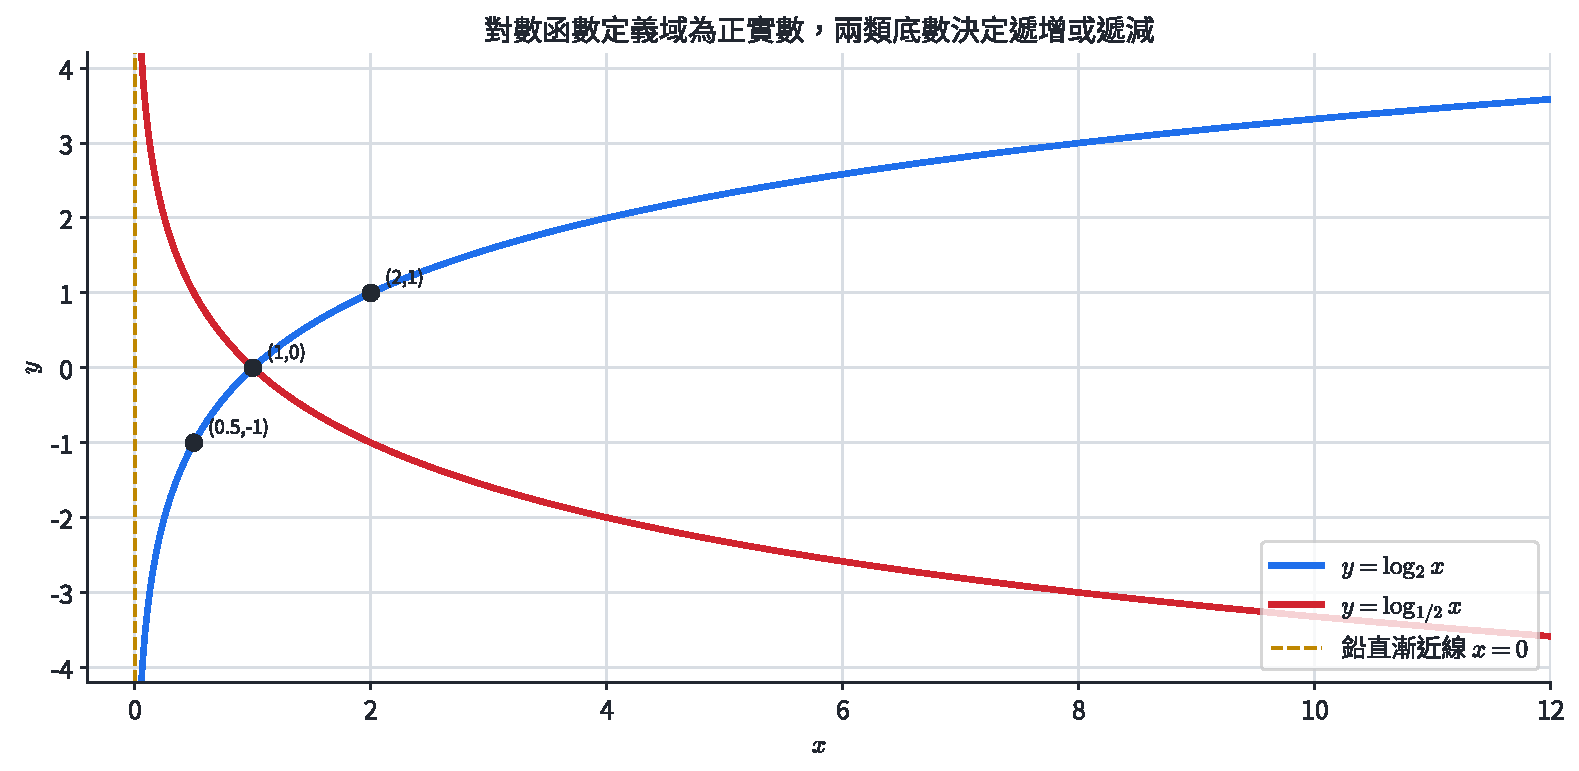
\includegraphics[width=0.9\linewidth,height=\textheight,keepaspectratio,alt={底數 2 與二分之一的對數圖形}]{assets/數B3-2-對數成長與衰退.pdf}
\caption{底數 2 與二分之一的對數圖形}
\end{figure}

圖中 \(y=\log_2x\) 通過 \((1,0)\)、\((2,1)\) 與 \((1/2,-1)\)；\(y=\log_{1/2}x=-\log_2x\) 與它關於 \(x\) 軸對稱。兩條曲線都只在 \(x>0\) 出現。

\subsection{7.2 對數方程式與不等式}\label{ux5c0dux6578ux65b9ux7a0bux5f0fux8207ux4e0dux7b49ux5f0f}

處理含對數的方程式時，先由每個真數列出正數條件，再使用對數律或單調性化簡。得到代數候選值後，以原來每個真數的條件篩選。

對 \(u,v>0\)：

\[
\log_a u=\log_a v\Longleftrightarrow u=v.
\]

不等式由增減性決定：

\[
\begin{aligned}
a>1 &: \quad \log_a u>\log_a v\Longleftrightarrow u>v,\\
0<a<1 &: \quad \log_a u>\log_a v\Longleftrightarrow u<v.
\end{aligned}
\]

\subsection{例 22｜由底數讀圖形特徵}\label{ux4f8b-22ux7531ux5e95ux6578ux8b80ux5716ux5f62ux7279ux5fb5}

對 \(f(x)=\log_{1/3}x\)：

\begin{itemize}
\tightlist
\item
  定義域為 \((0,\infty)\)，值域為 \(\mathbb R\)。
\item
  通過 \((1,0)\)。
\item
  因 \(0<1/3<1\)，函數遞減。
\item
  \(\log_{1/3}(1/3)=1\)，\(\log_{1/3}3=-1\)，所以還通過 \((1/3,1)\) 與 \((3,-1)\)。
\item
  \(x=0\) 是鉛直漸近線。
\end{itemize}

這些代數點和增減性已能確定圖形的主要形狀。

\subsection{例 23｜對數方程式的真數條件}\label{ux4f8b-23ux5c0dux6578ux65b9ux7a0bux5f0fux7684ux771fux6578ux689dux4ef6}

解

\[
\log_2(x-1)+\log_2(x-3)=3.
\]

真數條件為 \(x-1>0\) 且 \(x-3>0\)，合併得 \(x>3\)。利用乘法律：

\[
\log_2[(x-1)(x-3)]=3,
\]

\[
(x-1)(x-3)=2^3=8.
\]

展開得 \(x^2-4x-5=0\)，候選值為 \(x=5,-1\)。條件 \(x>3\) 保留 \(x=5\)。

\subsection{例 24｜底數小於 1 的對數不等式}\label{ux4f8b-24ux5e95ux6578ux5c0fux65bc-1-ux7684ux5c0dux6578ux4e0dux7b49ux5f0f}

解

\[
\log_{1/3}(2x-1)>-1.
\]

真數條件給出 \(x>1/2\)。又

\[
-1=\log_{1/3}3.
\]

因 \(\log_{1/3}x\) 遞減，所以

\[
2x-1<3,\qquad x<2.
\]

與定義域取交集，得

\[
\frac12<x<2.
\]

\subsection{例 25｜圖解、代數解與定義域一致}\label{ux4f8b-25ux5716ux89e3ux4ee3ux6578ux89e3ux8207ux5b9aux7fa9ux57dfux4e00ux81f4}

解

\[
\log(x-1)+\log(2x+1)=\log20.
\]

原真數條件為 \(x>1\) 與 \(x>-1/2\)，合併為 \(x>1\)。因此

\[
(x-1)(2x+1)=20,
\]

\[
2x^2-x-21=0,\qquad (2x-7)(x+3)=0.
\]

候選值為 \(x=7/2,-3\)，保留 \(x=7/2\)。

\begin{figure}
\centering
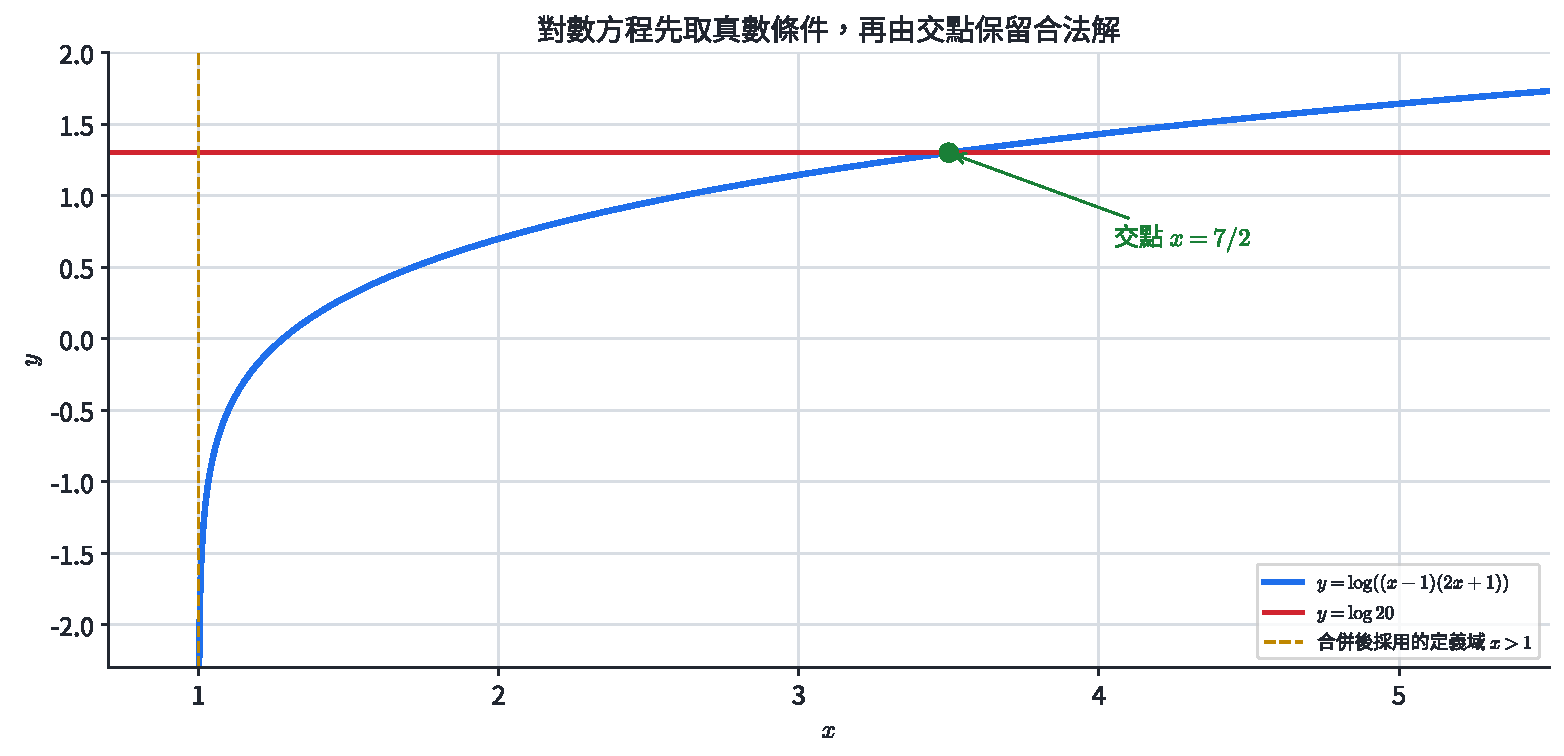
\includegraphics[width=0.9\linewidth,height=\textheight,keepaspectratio,alt={對數方程式的合法定義域與圖形交點}]{assets/數B3-2-對數方程與定義域.pdf}
\caption{對數方程式的合法定義域與圖形交點}
\end{figure}

圖中只在 \(x>1\) 畫出合併後的對數式，與水平線 \(y=\log20\) 的交點橫座標是 \(7/2\)，與代數篩選結果相同。

\subsection{7.3 分節練習}\label{ux5206ux7bc0ux7df4ux7fd2-6}

\begin{enumerate}
\def\labelenumi{\arabic{enumi}.}
\tightlist
\item
  寫出 \(y=\log_5x\) 的定義域、值域、漸近線、通過的固定點與增減性。
\item
  列出 \(y=\log_{1/4}x\) 在 \(x=1/4,1,4\) 時的座標，並指出圖形的增減性。
\item
  解 \(\log_3(x-2)=2\)。
\item
  解 \(\log_2x+\log_2(x-2)=3\)。
\item
  解 \(\log_{1/2}(x+1)\le-2\)。
\end{enumerate}

\subsection{7.4 分節練習解析}\label{ux5206ux7bc0ux7df4ux7fd2ux89e3ux6790-6}

\begin{enumerate}
\def\labelenumi{\arabic{enumi}.}
\tightlist
\item
  定義域 \((0,\infty)\)，值域 \(\mathbb R\)，鉛直漸近線 \(x=0\)，通過 \((1,0)\)；因 \(5>1\)，函數遞增。
\item
  \[
   \log_{1/4}\frac14=1,\qquad \log_{1/4}1=0,\qquad
   \log_{1/4}4=-1.
   \]
  對應點為 \((1/4,1)\)、\((1,0)\)、\((4,-1)\)，圖形遞減。
\item
  真數條件 \(x>2\)。由 \(x-2=3^2=9\)，得 \(x=11\)，符合條件。
\item
  真數條件 \(x>2\)。合併得 \(x(x-2)=8\)，即 \(x^2-2x-8=0\)，候選值 \(4,-2\)。保留 \(x=4\)。
\item
  真數條件 \(x>-1\)。又 \(-2=\log_{1/2}4\)，函數遞減，所以 \(x+1\ge4\)，得 \(x\ge3\)。這些值全部符合定義域。
\end{enumerate}

對數函數的圖形能將「已知倍率，反求指數」視覺化。橫線與對數圖的交點可讀出門檻時間，定義域則對應原始量必須為正。

\section{8. 指數函數與對數函數的關係}\label{ux6307ux6578ux51fdux6578ux8207ux5c0dux6578ux51fdux6578ux7684ux95dcux4fc2}

\subsection{8.1 互換輸入與輸出}\label{ux4e92ux63dbux8f38ux5165ux8207ux8f38ux51fa}

指數關係

\[
y=a^x
\]

等價於

\[
x=\log_a y.
\]

互換變數名稱得 \(y=\log_a x\)。因此 \(f(x)=a^x\) 與 \(f^{-1}(x)=\log_a x\) 互為反函數。若 \((u,v)\) 在 \(y=a^x\) 上，則 \((v,u)\) 在 \(y=\log_a x\) 上；座標互換對應關於 \(y=x\) 鏡射。

\begin{figure}
\centering
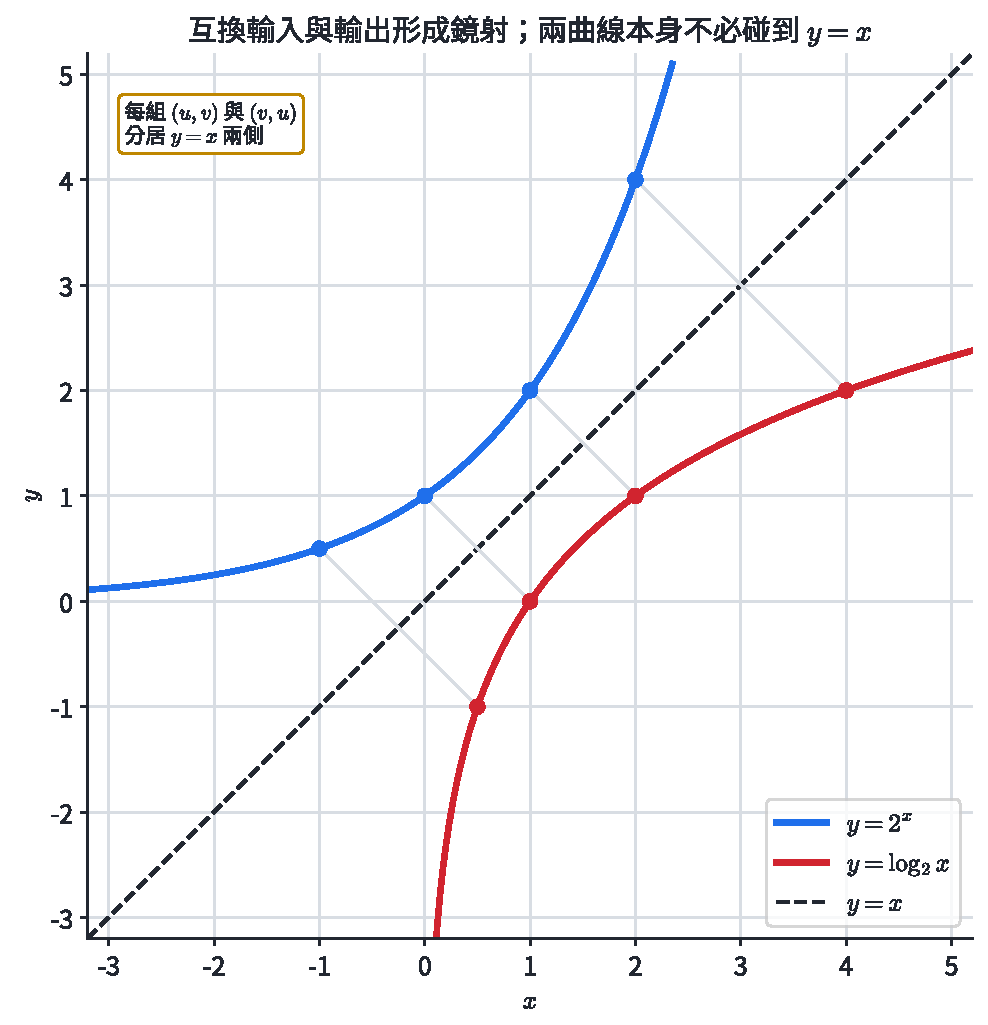
\includegraphics[width=0.84\linewidth,height=\textheight,keepaspectratio,alt={指數函數與對數函數的成對點及鏡射}]{assets/數B3-2-指數對數互為反函數.pdf}
\caption{指數函數與對數函數的成對點及鏡射}
\end{figure}

圖中 \((-1,1/2)\)、\((0,1)\)、\((1,2)\)、\((2,4)\) 在 \(y=2^x\) 上，互換座標後的四點在 \(y=\log_2x\) 上。連接每對點的線段都垂直於 \(y=x\)，中點落在 \(y=x\) 上。

鏡射關係描述成對點；兩條曲線是否與 \(y=x\) 相交，另由 \(2^x=x\) 決定。以三個區間可驗證 \(2^x>x\)：

\begin{enumerate}
\def\labelenumi{\arabic{enumi}.}
\tightlist
\item
  \(x<0\) 時，\(2^x>0>x\)。
\item
  \(0\le x<1\) 時，\(2^x\ge1>x\)；\(x=1\) 時，\(2^1=2>1\)。
\item
  \(x>1\) 時，取正整數 \(n\) 使 \(n\le x<n+1\)。由 \(2^x\) 遞增且 \(2^n\ge n+1\)（可以數學歸納法驗證），得
  \[
  2^x\ge2^n\ge n+1>x.
  \]
\end{enumerate}

因此方程式 \(2^x=x\) 無解；\(y=2^x\)、\(y=\log_2x\) 與鏡面 \(y=x\) 都沒有交點。圖中的間隔是代數不等式的精確結果。

\subsection{例 26｜由指數圖上的點得到對數圖上的點}\label{ux4f8b-26ux7531ux6307ux6578ux5716ux4e0aux7684ux9edeux5f97ux5230ux5c0dux6578ux5716ux4e0aux7684ux9ede}

因 \(3^{-2}=1/9\)、\(3^1=3\)，所以指數圖 \(y=3^x\) 上有點

\[
\left(-2,\frac19\right),\qquad(1,3).
\]

互換座標後，對數圖 \(y=\log_3x\) 上有點

\[
\left(\frac19,-2\right),\qquad(3,1).
\]

\subsection{例 27｜平移後的反函數}\label{ux4f8b-27ux5e73ux79fbux5f8cux7684ux53cdux51fdux6578}

設

\[
f(x)=3^{x-2}+1.
\]

令 \(y=3^{x-2}+1\)，互換 \(x,y\)：

\[
x=3^{y-2}+1.
\]

由 \(x-1=3^{y-2}\) 得

\[
\log_3(x-1)=y-2,\qquad
f^{-1}(x)=2+\log_3(x-1).
\]

反函數的定義域 \(x>1\) 正是原函數值域 \((1,\infty)\)。

\subsection{8.2 取對數後的直線資料}\label{ux53d6ux5c0dux6578ux5f8cux7684ux76f4ux7ddaux8cc7ux6599}

若資料符合

\[
Q(t)=Q_0a^t,\qquad Q_0>0,\quad a>0,\quad a\ne1,
\]

兩邊取常用對數：

\[
\log Q=\log Q_0+t\log a.
\]

以 \(t\) 為橫軸、\(\log Q\) 為縱軸時，得到直線，截距是 \(\log Q_0\)，斜率是 \(\log a\)。斜率為正對應 \(a>1\)，斜率為負對應 \(0<a<1\)。

\begin{figure}
\centering
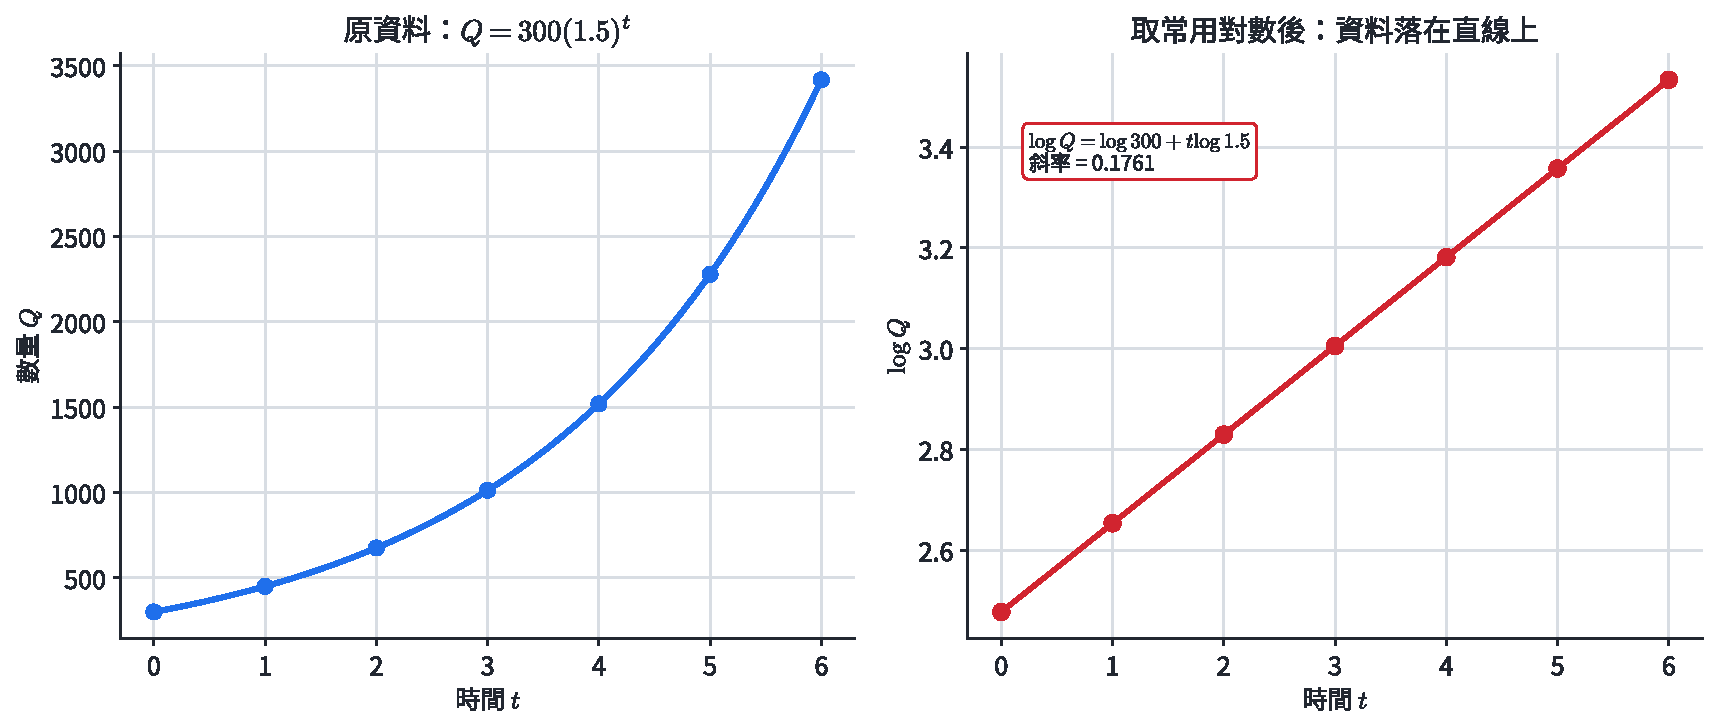
\includegraphics[width=0.94\linewidth,height=\textheight,keepaspectratio,alt={指數資料取常用對數後形成直線}]{assets/數B3-2-指數資料取對數.pdf}
\caption{指數資料取常用對數後形成直線}
\end{figure}

左圖資料符合 \(Q=300(1.5)^t\)；右圖的每個點縱座標改為 \(\log Q\)，所有點落在

\[
\log Q=\log300+t\log1.5
\]

上。圖中斜率約 \(0.1761\)，和數值計算 \(\log1.5\) 一致。

\subsection{例 28｜由對數直線回復指數模型}\label{ux4f8b-28ux7531ux5c0dux6578ux76f4ux7ddaux56deux5fa9ux6307ux6578ux6a21ux578b}

某資料取常用對數後滿足

\[
\log Q=2.3010+0.07918t.
\]

由 \(2.3010\approx\log200\)、\(0.07918\approx\log1.2\)，得

\[
\log Q=\log200+t\log1.2
=\log[200(1.2)^t].
\]

因此

\[
Q=200(1.2)^t.
\]

截距回復初值 \(200\)，斜率回復每期倍率 \(1.2\)。

\subsection{8.3 分節練習}\label{ux5206ux7bc0ux7df4ux7fd2-7}

\begin{enumerate}
\def\labelenumi{\arabic{enumi}.}
\tightlist
\item
  寫出 \(f(x)=5^x\) 的反函數，並說明兩函數的定義域與值域如何互換。
\item
  已知 \((2,9)\) 在 \(y=3^x\) 上。寫出對應在 \(y=\log_3x\) 上的點，並求兩點中點。
\item
  對 \(y=2^x\) 與 \(y=\log_2x\)，說明為何鏡射對應不會強制兩曲線通過 \(y=x\)，並將實數分成 \(x<0\)、\(0\le x\le1\)、\(x>1\) 驗證交點數。
\item
  求 \(f(x)=2^{x+1}-3\) 的反函數與定義域。
\item
  某資料在 \(t=0,1,2\) 時依序為 \(200,260,338\)。若固定倍率模型成立，寫出 \(Q(t)\) 與 \(\log Q\) 的直線形式，並求連續時間下 \(Q\) 達到 \(1000\) 的時間。
\end{enumerate}

\subsection{8.4 分節練習解析}\label{ux5206ux7bc0ux7df4ux7fd2ux89e3ux6790-7}

\begin{enumerate}
\def\labelenumi{\arabic{enumi}.}
\tightlist
\item
  \(f^{-1}(x)=\log_5x\)。\(5^x\) 的定義域 \(\mathbb R\) 成為反函數的值域；\(5^x\) 的值域 \((0,\infty)\) 成為反函數的定義域。
\item
  互換座標得 \((9,2)\)。兩點中點為 \((11/2,11/2)\)，位於 \(y=x\)。
\item
  鏡射規則是 \((u,v)\leftrightarrow(v,u)\)，是成對點的對應。交點需另滿足 \(2^x=x\)。\(x<0\) 時 \(2^x>0>x\)；\(0\le x<1\) 時 \(2^x\ge1>x\)，\(x=1\) 時 \(2>1\)；\(x>1\) 時取 \(n\le x<n+1\)，利用 \(2^n\ge n+1\) 得 \(2^x\ge2^n\ge n+1>x\)。所有區間都有 \(2^x>x\)，所以交點數為 \(0\)。
\item
  令 \(y=2^{x+1}-3\)，互換後得 \(x+3=2^{y+1}\)，所以
  \[
  f^{-1}(x)=\log_2(x+3)-1,\qquad x>-3.
  \]
\item
  相鄰比值均為 \(1.3\)，所以
  \[
  Q(t)=200(1.3)^t,\qquad
  \log Q=\log200+t\log1.3.
  \]
  令 \(Q=1000\)：
  \[
  t=\frac{\log5}{\log1.3}\approx6.13.
  \]
  所以連續模型約在 \(6.13\) 期達到 \(1000\)。
\end{enumerate}

反函數將「由時間求數量」改成「由數量求時間」；取對數將指數曲線轉為直線。這兩個觀點共同支持資料判讀、參數估計與門檻時間預測。

\section{9. 章末代表題}\label{ux7ae0ux672bux4ee3ux8868ux984c}

\subsection{9.1 基礎與變式}\label{ux57faux790eux8207ux8b8aux5f0f}

\begin{enumerate}
\def\labelenumi{\arabic{enumi}.}
\tightlist
\item
  對指數函數 \(f(x)=(1/5)^x\)，寫出底數條件、定義域、值域、增減性，並求 \(f(-2)\)。
\item
  某測量量連續四期為 \(96,144,216,324\)。檢查固定倍率，並寫出以第一筆為 \(Q_0\) 的模型。
\item
  解方程式 \(2^{x+2}=16^{x-1}\)。
\item
  解不等式 \(3^{2x}-10\cdot3^x+9\le0\)。
\item
  某物質初始質量為 \(480\text{ g}\)，半衰期為 \(18\) 年。在此衰退模型下，求 \(45\) 年後質量。
\item
  本金 \(160{,}000\) 元，名義年利率 \(2.4\%\)，每月複利。求 \(3\) 年後本利和。
\item
  化簡
  \[
  \log24+\log15-\log9-\log4.
  \]
\item
  解方程式 \(\log_4(x-1)=\log_2 3\)。
\item
  某量依 \(Q(t)=900e^{0.04t}\) 連續成長。求翻倍時間。
\item
  兩聲音的聲強級相差 \(24\) 分貝。求強聲與弱聲的聲強比。
\item
  對 \(y=\log_2(x-3)+1\)，寫出定義域、值域、鉛直漸近線、增減性，並找一個整數座標點。
\item
  解不等式 \(\log_{1/2}(x-1)\le-2\)。
\end{enumerate}

\subsection{9.2 跨節整合}\label{ux8de8ux7bc0ux6574ux5408}

\begin{enumerate}
\def\labelenumi{\arabic{enumi}.}
\setcounter{enumi}{12}
\item
  某藻類在實驗前 \(20\) 小時的資料如下：

  {\def\LTcaptype{none} % do not increment counter
  \begin{longtable}[]{@{}rrrr@{}}
  \toprule\noalign{}
  \(t\) （小時） & 0 & 4 & 8 \\
  \midrule\noalign{}
  \endhead
  \bottomrule\noalign{}
  \endlastfoot
  數量 \(Q\) & 120 & 180 & 270 \\
  \end{longtable}
  }

  假設每 \(4\) 小時倍率穩定：

  \begin{itemize}
  \tightlist
  \item
    \begin{enumerate}
    \def\labelenumii{(\alph{enumii})}
    \tightlist
    \item
      建立連續時間模型。
    \end{enumerate}
  \item
    \begin{enumerate}
    \def\labelenumii{(\alph{enumii})}
    \setcounter{enumii}{1}
    \tightlist
    \item
      求數量超過 \(600\) 的連續時間門檻。
    \end{enumerate}
  \item
    \begin{enumerate}
    \def\labelenumii{(\alph{enumii})}
    \setcounter{enumii}{2}
    \tightlist
    \item
      若只每 \(4\) 小時記錄，首次超過 \(600\) 的記錄時間為何？
    \end{enumerate}
  \item
    \begin{enumerate}
    \def\labelenumii{(\alph{enumii})}
    \setcounter{enumii}{3}
    \tightlist
    \item
      寫出 \(\log Q\) 對 \(t\) 的直線式。
    \end{enumerate}
  \end{itemize}
\item
  將 \(200{,}000\) 元存入年期存款，每季利率 \(1.2\%\)，利息每季加入本金。

  \begin{itemize}
  \tightlist
  \item
    \begin{enumerate}
    \def\labelenumii{(\alph{enumii})}
    \tightlist
    \item
      寫出 \(t\) 年後本利和 \(A(t)\)。
    \end{enumerate}
  \item
    \begin{enumerate}
    \def\labelenumii{(\alph{enumii})}
    \setcounter{enumii}{1}
    \tightlist
    \item
      求本利和首次超過 \(250{,}000\) 元的連續時間。
    \end{enumerate}
  \item
    \begin{enumerate}
    \def\labelenumii{(\alph{enumii})}
    \setcounter{enumii}{2}
    \tightlist
    \item
      若銀行只在每季末計入利息，至少需要幾季？
    \end{enumerate}
  \end{itemize}
\item
  地震能量模型為 \(\log E=11.8+1.5M\)。A地震規模為 \(6.8\)，B地震規模為 \(5.4\)。

  \begin{itemize}
  \tightlist
  \item
    \begin{enumerate}
    \def\labelenumii{(\alph{enumii})}
    \tightlist
    \item
      求兩地震的 \(\log E\) 差。
    \end{enumerate}
  \item
    \begin{enumerate}
    \def\labelenumii{(\alph{enumii})}
    \setcounter{enumii}{1}
    \tightlist
    \item
      求能量比 \(E_A/E_B\)。
    \end{enumerate}
  \item
    \begin{enumerate}
    \def\labelenumii{(\alph{enumii})}
    \setcounter{enumii}{2}
    \tightlist
    \item
      用「規模差」與「能量倍率」說明對數尺度壓縮數值範圍的機制。
    \end{enumerate}
  \end{itemize}
\item
  某生物量資料為

  {\def\LTcaptype{none} % do not increment counter
  \begin{longtable}[]{@{}rrrr@{}}
  \toprule\noalign{}
  \(t\) （天） & 0 & 2 & 4 \\
  \midrule\noalign{}
  \endhead
  \bottomrule\noalign{}
  \endlastfoot
  \(Q\) （單位） & 80 & 120 & 180 \\
  \end{longtable}
  }

  假設每 \(2\) 天倍率穩定：

  \begin{itemize}
  \tightlist
  \item
    \begin{enumerate}
    \def\labelenumii{(\alph{enumii})}
    \tightlist
    \item
      建立 \(Q(t)\)。
    \end{enumerate}
  \item
    \begin{enumerate}
    \def\labelenumii{(\alph{enumii})}
    \setcounter{enumii}{1}
    \tightlist
    \item
      寫出 \(\log Q\) 對 \(t\) 的直線，並指出斜率與截距。
    \end{enumerate}
  \item
    \begin{enumerate}
    \def\labelenumii{(\alph{enumii})}
    \setcounter{enumii}{2}
    \tightlist
    \item
      求 \(Q=300\) 的連續時間。
    \end{enumerate}
  \item
    \begin{enumerate}
    \def\labelenumii{(\alph{enumii})}
    \setcounter{enumii}{3}
    \tightlist
    \item
      將點 \((2,120)\) 視為映射 \(t\mapsto Q\)的點，寫出反映射圖上的對應點，並解釋其單位意義。
    \end{enumerate}
  \end{itemize}
\end{enumerate}

\section{10. 完整詳解}\label{ux5b8cux6574ux8a73ux89e3}

\subsection{第 1 題}\label{ux7b2c-1-ux984c}

底數 \(1/5\) 滿足 \(a>0\) 且 \(a\ne1\)。定義域為 \(\mathbb R\)，值域為 \((0,\infty)\)。由 \(0<1/5<1\)，函數遞減。

\[
f(-2)=\left(\frac15\right)^{-2}=25.
\]

\subsection{第 2 題}\label{ux7b2c-2-ux984c}

相鄰比值為

\[
\frac{144}{96}=\frac{216}{144}=\frac{324}{216}=1.5.
\]

因此固定倍率是 \(1.5\)，模型為

\[
Q_n=96(1.5)^n.
\]

\subsection{第 3 題}\label{ux7b2c-3-ux984c}

\(16=2^4\)，所以

\[
2^{x+2}=2^{4x-4}.
\]

由一對一性，\(x+2=4x-4\)，得

\[
x=2.
\]

代回時兩邊均為 \(16\)。

\subsection{第 4 題}\label{ux7b2c-4-ux984c}

令 \(u=3^x>0\)，則

\[
u^2-10u+9=(u-1)(u-9)\le0.
\]

二次式在兩根之間非正，所以 \(1\le u\le9\)，也就是

\[
1\le3^x\le3^2.
\]

\(3^x\) 遞增，故

\[
0\le x\le2.
\]

\subsection{第 5 題}\label{ux7b2c-5-ux984c}

\(45\) 年包含 \(45/18=2.5\) 個半衰期，所以

\[
M(45)=480\left(\frac12\right)^{45/18}
=480\left(\frac12\right)^{2.5}
\approx84.85\text{ g}.
\]

結果為正且低於經過兩個半衰期時的 \(120\text{ g}\)，與衰退方向一致。

\subsection{第 6 題}\label{ux7b2c-6-ux984c}

每月利率為 \(0.024/12=0.002\)，\(3\) 年共 \(36\) 期：

\[
A=160000(1.002)^{36}\approx171932.49.
\]

本利和約為 \(171{,}932\) 元。

\subsection{第 7 題}\label{ux7b2c-7-ux984c}

所有真數均為正，可合併：

\[
\log24+\log15-\log9-\log4
=\log\frac{24\cdot15}{9\cdot4}
=\log10=1.
\]

\subsection{第 8 題}\label{ux7b2c-8-ux984c}

將右邊改寫為底數 \(4\)：

\[
\log_2 3=\frac{\log_4 3}{\log_4 2}=2\log_4 3=\log_4 9.
\]

因此

\[
\log_4(x-1)=\log_4 9,\qquad x-1=9,\qquad x=10.
\]

真數 \(x-1=9>0\)，符合定義域。

\subsection{第 9 題}\label{ux7b2c-9-ux984c}

翻倍時 \(T\) 滿足

\[
900e^{0.04T}=1800.
\]

約去初值並取自然對數：

\[
0.04T=\ln2,\qquad
T=\frac{\ln2}{0.04}\approx17.33.
\]

時間單位與模型中 \(t\) 的單位相同。

\subsection{第 10 題}\label{ux7b2c-10-ux984c}

令聲強比為 \(R\)，則

\[
24=10\log R,\qquad \log R=2.4.
\]

\[
R=10^{2.4}\approx251.2.
\]

所以強聲的聲強約是弱聲的 \(251\) 倍。

\subsection{第 11 題}\label{ux7b2c-11-ux984c}

真數條件 \(x-3>0\) 給出定義域 \((3,\infty)\)；值域仍為 \(\mathbb R\)；鉛直漸近線由 \(x=0\) 向右平移 \(3\)，成為 \(x=3\)。底數 \(2>1\)，圖形遞增。取 \(x=4\)：

\[
y=\log_2(4-3)+1=1,
\]

所以 \((4,1)\) 是一個整數座標點。

\subsection{第 12 題}\label{ux7b2c-12-ux984c}

真數條件為 \(x>1\)。又

\[
-2=\log_{1/2}4.
\]

因 \(\log_{1/2}x\) 遞減，

\[
x-1\ge4,\qquad x\ge5.
\]

這個區間已包含在 \(x>1\) 中，故解為 \([5,\infty)\)。

\subsection{第 13 題｜跨節整合}\label{ux7b2c-13-ux984cux8de8ux7bc0ux6574ux5408}

\begin{enumerate}
\def\labelenumi{(\alph{enumi})}
\tightlist
\item
  每 \(4\) 小時的比值為
\end{enumerate}

\[
\frac{180}{120}=\frac{270}{180}=1.5.
\]

連續時間模型為

\[
Q(t)=120(1.5)^{t/4}.
\]

\begin{enumerate}
\def\labelenumi{(\alph{enumi})}
\setcounter{enumi}{1}
\tightlist
\item
  求 \(Q(t)>600\)：
\end{enumerate}

\[
120(1.5)^{t/4}>600
\Longleftrightarrow
(1.5)^{t/4}>5.
\]

由 \(1.5>1\)，取對數得

\[
t>\frac{4\log5}{\log1.5}\approx15.88.
\]

連續模型約在 \(15.88\) 小時越過 \(600\)。

\begin{enumerate}
\def\labelenumi{(\alph{enumi})}
\setcounter{enumi}{2}
\tightlist
\item
  每 \(4\) 小時記錄時，下一個記錄點是 \(t=16\)：
\end{enumerate}

\[
Q(16)=120(1.5)^4=607.5>600.
\]

所以首次記錄到超過門檻是 \(16\) 小時。

\begin{enumerate}
\def\labelenumi{(\alph{enumi})}
\setcounter{enumi}{3}
\tightlist
\item
  取常用對數：
\end{enumerate}

\[
\log Q=\log120+\frac{t}{4}\log1.5.
\]

直線截距是 \(\log120\)，斜率是 \(\log1.5/4\)。

\subsection{第 14 題｜跨節整合}\label{ux7b2c-14-ux984cux8de8ux7bc0ux6574ux5408}

\begin{enumerate}
\def\labelenumi{(\alph{enumi})}
\tightlist
\item
  每年 \(4\) 季，\(t\) 年共 \(4t\) 期，所以
\end{enumerate}

\[
A(t)=200000(1.012)^{4t}.
\]

\begin{enumerate}
\def\labelenumi{(\alph{enumi})}
\setcounter{enumi}{1}
\tightlist
\item
  求 \(A(t)>250000\)：
\end{enumerate}

\[
(1.012)^{4t}>1.25.
\]

取對數得

\[
t>\frac{\log1.25}{4\log1.012}\approx4.677\text{ 年}.
\]

\begin{enumerate}
\def\labelenumi{(\alph{enumi})}
\setcounter{enumi}{2}
\tightlist
\item
  令季數為整數 \(n\)，條件為
\end{enumerate}

\[
n>\frac{\log1.25}{\log1.012}\approx18.707.
\]

所以至少需要 \(19\) 季。\(19\) 季是 \(4.75\) 年，與連續門檻 \(4.677\) 年的先後關係一致。

\subsection{第 15 題｜跨節整合}\label{ux7b2c-15-ux984cux8de8ux7bc0ux6574ux5408}

\begin{enumerate}
\def\labelenumi{(\alph{enumi})}
\tightlist
\item
  兩式相減時常數 \(11.8\) 消去：
\end{enumerate}

\[
\log E_A-\log E_B
=1.5(6.8-5.4)=2.1.
\]

\begin{enumerate}
\def\labelenumi{(\alph{enumi})}
\setcounter{enumi}{1}
\tightlist
\item
  用商的對數律：
\end{enumerate}

\[
\log\frac{E_A}{E_B}=2.1,\qquad
\frac{E_A}{E_B}=10^{2.1}\approx125.9.
\]

A 地震釋放的能量約為 B 的 \(126\) 倍。

\begin{enumerate}
\def\labelenumi{(\alph{enumi})}
\setcounter{enumi}{2}
\tightlist
\item
  規模只相差 \(1.4\)，對數能量差為 \(2.1\)，回到原能量尺度就是乘上 \(10^{2.1}\)。對數把原本的倍率 \(125.9\) 轉成加法差 \(2.1\)，因此可以在短尺度上表示跨越多個數量級的能量。
\end{enumerate}

\subsection{第 16 題｜跨節整合}\label{ux7b2c-16-ux984cux8de8ux7bc0ux6574ux5408}

\begin{enumerate}
\def\labelenumi{(\alph{enumi})}
\tightlist
\item
  每 \(2\) 天的比值為
\end{enumerate}

\[
\frac{120}{80}=\frac{180}{120}=1.5.
\]

因此

\[
Q(t)=80(1.5)^{t/2}.
\]

\begin{enumerate}
\def\labelenumi{(\alph{enumi})}
\setcounter{enumi}{1}
\tightlist
\item
  取常用對數：
\end{enumerate}

\[
\log Q=\log80+\frac{\log1.5}{2}t.
\]

截距是 \(\log80\)，斜率是 \(\log1.5/2\)。斜率為正，對應原數據成長。

\begin{enumerate}
\def\labelenumi{(\alph{enumi})}
\setcounter{enumi}{2}
\tightlist
\item
  令 \(Q=300\)：
\end{enumerate}

\[
80(1.5)^{t/2}=300,\qquad
(1.5)^{t/2}=3.75.
\]

\[
t=\frac{2\log3.75}{\log1.5}\approx6.52\text{ 天}.
\]

\begin{enumerate}
\def\labelenumi{(\alph{enumi})}
\setcounter{enumi}{3}
\tightlist
\item
  反映射互換輸入與輸出，所以對應點是 \((120,2)\)。原點 \((2\text{ 天},120\text{ 單位})\) 表示由時間預測生物量；反映射的 \((120\text{ 單位},2\text{ 天})\) 表示由目標生物量反求時間。座標數值互換時，物理單位也随輸入與輸出角色互換。
\end{enumerate}

\section{11. 核心整理}\label{ux6838ux5fc3ux6574ux7406}

\subsection{11.1 指數函數與模型}\label{ux6307ux6578ux51fdux6578ux8207ux6a21ux578b}

\begin{itemize}
\tightlist
\item
  \(f(x)=a^x\) 的條件是 \(a>0\)、\(a\ne1\)；定義域 \(\mathbb R\)，值域 \((0,\infty)\)，通過 \((0,1)\)。
\item
  \(a>1\) 時遞增；\(0<a<1\) 時遞減；\(y=0\) 是水平漸近線。
\item
  每 \(h\) 單位時間乘上 \(b\) 的模型是 \(Q(t)=Q_0b^{t/h}\)。
\item
  百分率成長 \(r\) 的倍率是 \(1+r\)；百分率衰退 \(r\) 的保留率是 \(1-r\)。
\item
  單利每期增加固定金額：\(A=P(1+nr)\)；複利每期乘上固定倍率：\(A=P(1+r)^n\)。
\end{itemize}

\subsection{11.2 對數定義與運算}\label{ux5c0dux6578ux5b9aux7fa9ux8207ux904bux7b97}

\[
a^b=r\Longleftrightarrow b=\log_a r,\qquad
a>0,\quad a\ne1,\quad r>0.
\]

\[
\log_a(MN)=\log_aM+\log_aN,\qquad
\log_a\frac MN=\log_aM-\log_aN,\qquad
\log_a(M^k)=k\log_aM.
\]

\[
\log_a r=\frac{\log_c r}{\log_c a}.
\]

對數方程式的每個真數都需大於 \(0\)。真數條件先確定可用區間，代數化簡產生候選值，最後以條件篩選。

\subsection{11.3 對數函數、反函數與資料}\label{ux5c0dux6578ux51fdux6578ux53cdux51fdux6578ux8207ux8cc7ux6599}

\begin{itemize}
\tightlist
\item
  \(y=\log_a x\) 的定義域 \((0,\infty)\)，值域 \(\mathbb R\)，通過 \((1,0)\)，\(x=0\) 是鉛直漸近線。
\item
  \(a>1\) 時遞增；\(0<a<1\) 時遞減，不等式的大小關係由這個單調性決定。
\item
  \(y=a^x\) 與 \(y=\log_ax\) 互為反函數，\((u,v)\) 與 \((v,u)\) 關於 \(y=x\) 對應。兩曲線是否與 \(y=x\) 相交，由 \(a^x=x\) 另行決定。
\item
  若 \(Q=Q_0a^t\)，則 \(\log Q=\log Q_0+t\log a\)。對數圖的截距回復初值，斜率回復每期倍率。
\item
  門檻時間由 \(t=\log(Q_*/Q_0)/\log a\) 反求；連續越過時間與離散觀測時間需依量測間隔分別回答。
\end{itemize}

指數模型的有效性來自固定倍率的證據。建模後同時保留初值、倍率、時間單位與適用區間，才能將計算結果解釋成具體的數量與時間。


\end{document}
